\def\year{2021}\relax
%File: formatting-instructions-latex-2021.tex
%release 2021.1


% \documentclass[letterpaper]{article} % DO NOT CHANGE THIS
% \usepackage{aaai21}  % DO NOT CHANGE THIS
% \usepackage{times}  % DO NOT CHANGE THIS
% \usepackage{helvet} % DO NOT CHANGE THIS
% \usepackage{courier}  % DO NOT CHANGE THIS
% \usepackage[hyphens]{url}  % DO NOT CHANGE THIS
% \usepackage{graphicx} % DO NOT CHANGE THIS
% \urlstyle{rm} % DO NOT CHANGE THIS
% \def\UrlFont{\rm}  % DO NOT CHANGE THIS
% \usepackage{natbib}  % DO NOT CHANGE THIS AND DO NOT ADD ANY OPTIONS TO IT
% \usepackage{caption} % DO NOT CHANGE THIS AND DO NOT ADD ANY OPTIONS TO IT

% \usepackage{multirow}
% \usepackage{booktabs}



% \frenchspacing  % DO NOT CHANGE THIS
% \setlength{\pdfpagewidth}{8.5in}  % DO NOT CHANGE THIS
% \setlength{\pdfpageheight}{11in}  % DO NOT CHANGE THIS

\documentclass{article}
\pdfpagewidth=8.5in
\pdfpageheight=11in

\usepackage{kr}

% Use the postscript times font!
\usepackage{times}
\usepackage{soul}
\usepackage{url}
\usepackage[hidelinks]{hyperref}
\usepackage[utf8]{inputenc}
\usepackage[small]{caption}
\usepackage{graphicx}
\usepackage{amsmath}
\usepackage{amsthm}
\usepackage{booktabs}
% \usepackage{algorithm}
\usepackage{algorithmic}
\urlstyle{same}

% the following package is optional:
%\usepackage{latexsym}

% See https://www.overleaf.com/learn/latex/theorems_and_proofs
% for a nice explanation of how to define new theorems, but keep
% in mind that the amsthm package is already included in this
% template and that you must *not* alter the styling.
\newtheorem{example}{Example}


%\nocopyright
%PDF Info Is REQUIRED.
% For /Author, add all authors within the parentheses, separated by commas. No accents or commands.
% For /Title, add Title in Mixed Case. No accents or commands. Retain the parentheses.
\pdfinfo{
/TemplateVersion (KR.2021.0)
 %Leave this
/Title (Safe Learning of Lifted Action Models)
% Put your actual complete title (no codes, scripts, shortcuts, or LaTeX commands) within the parentheses in mixed case
% Leave the space between \Title and the beginning parenthesis alone
/Author (Brendan Juba, Hai S. Le, Roni Stern)
}
% Put your actual complete list of authors (no codes, scripts, shortcuts, or LaTeX commands) within the parentheses in mixed case.
% Each author should be only by a comma. If the name contains accents, remove them. If there are any LaTeX commands,
% remove them.

% DISALLOWED PACKAGES
% \usepackage{authblk} -- This package is specifically forbidden
% \usepackage{balance} -- This package is specifically forbidden
% \usepackage{color (if used in text)
% \usepackage{CJK} -- This package is specifically forbidden
% \usepackage{float} -- This package is specifically forbidden
% \usepackage{flushend} -- This package is specifically forbidden
% \usepackage{fontenc} -- This package is specifically forbidden
% \usepackage{fullpage} -- This package is specifically forbidden
% \usepackage{geometry} -- This package is specifically forbidden
% \usepackage{grffile} -- This package is specifically forbidden
% \usepackage{hyperref} -- This package is specifically forbidden
% \usepackage{navigator} -- This package is specifically forbidden
% (or any other package that embeds links such as navigator or hyperref)
% \indentfirst} -- This package is specifically forbidden
% \layout} -- This package is specifically forbidden
% \multicol} -- This package is specifically forbidden
% \nameref} -- This package is specifically forbidden
% \usepackage{savetrees} -- This package is specifically forbidden
% \usepackage{setspace} -- This package is specifically forbidden
% \usepackage{stfloats} -- This package is specifically forbidden
% \usepackage{tabu} -- This package is specifically forbidden
% \usepackage{titlesec} -- This package is specifically forbidden
% \usepackage{tocbibind} -- This package is specifically forbidden
% \usepackage{ulem} -- This package is specifically forbidden
% \usepackage{wrapfig} -- This package is specifically forbidden
% DISALLOWED COMMANDS
% \nocopyright -- Your paper will not be published if you use this command
% \addtolength -- This command may not be used
% \balance -- This command may not be used
% \baselinestretch -- Your paper will not be published if you use this command
% \clearpage -- No page breaks of any kind may be used for the final version of your paper
% \columnsep -- This command may not be used
% \newpage -- No page breaks of any kind may be used for the final version of your paper
% \pagebreak -- No page breaks of any kind may be used for the final version of your paperr
% \pagestyle -- This command may not be used
% \tiny -- This is not an acceptable font size.
% \vspace{- -- No negative value may be used in proximity of a caption, figure, table, section, subsection, subsubsection, or reference
% \vskip{- -- No negative value may be used to alter spacing above or below a caption, figure, table, section, subsection, subsubsection, or reference



\setcounter{secnumdepth}{2} %May be changed to 1 or 2 if section numbers are desired.


\usepackage{xspace}
\usepackage[linesnumbered,ruled,vlined]{algorithm2e}
\usepackage{paralist}
\usepackage{multirow}

\newtheorem{theorem}{Theorem}
\newtheorem{observation}{Observation}
\newtheorem{corollary}{Corollary}
\newtheorem{lemma}{Lemma}
\newtheorem{definition}{Definition}


\newcommand{\tuple}[1]{\ensuremath{\left \langle #1 \right \rangle }}
\newcommand{\pre}{\textit{pre}}
\newcommand{\params}{\textit{params}}
\newcommand{\eff}{\textit{eff}}
\newcommand{\name}{\textit{name}}
\newcommand{\type}{\textit{type}}
\newcommand{\cnf}{\textit{CNF}}
\newcommand{\conj}{\textit{Conj}}
\newcommand{\realm}{\ensuremath{M^*}\xspace}
\newcommand{\liftf}{F}
\newcommand{\liftl}{L}
\newcommand{\lifta}{A}
\newcommand{\sam}{\textit{SAM}\xspace}
\newcommand{\sgam}{\textit{SGAM}\xspace}
\newcommand{\bindings}{\textit{bindings}}
\newcommand{\iseff}{\text{IsEff}}
\newcommand{\ispre}{\text{IsPre}}

\usepackage{color}
%\usepackage{subcaption}

% \newcommand\mycommfont[1]{\footnotesize\textcolor{blue}{#1}}
% \SetCommentSty{mycommfont}

%
% Add comments in the text
%
% \newboolean{showcomments}
% \setboolean{showcomments}{true}
% %\setboolean{showcomments}{false}

% \ifthenelse{\boolean{showcomments}}
%   {\newcommand{\nb}[3]{
%   {\color{#2}\small\fbox{\bfseries\sffamily\scriptsize#1}}
%   {\color{#2}\sffamily\small$\triangleright~$\textit{\small #3}$~\triangleleft$}
%   }
%   }
%   {\newcommand{\nb}[3]{}
%   }
% \newcommand\brendan[1]{\nb{\textbf{Brendan:}}{green}{#1}}
% \newcommand\hai[1]{\nb{\textbf{Hai:}}{blue}{#1}}
% \newcommand\roni[1]{\nb{\textbf{Roni:}}{red}{#1}}



% \newcommand\mycommfont[1]{\footnotesize\textcolor{blue}{#1}}
% \SetCommentSty{mycommfont}

% The file aaai21.sty is the style file for AAAI Press
% proceedings, working notes, and technical reports.
%

% Title

% Your title must be in mixed case, not sentence case.
% That means all verbs (including short verbs like be, is, using,and go),
% nouns, adverbs, adjectives should be capitalized, including both words in hyphenated terms, while
% articles, conjunctions, and prepositions are lower case unless they
% directly follow a colon or long dash

\title{Safe Learning of Lifted Action Models\thanks{This is the KR 2021 proceedings version. See the associated technical report arXiv:2107.04169 [cs.AI] for full proofs.}}
% \author{Submission \#342
%     % %Authors
%     % % All authors must be in the same font size and format.
%     % Written by AAAI Press Staff\textsuperscript{\rm 1}\thanks{With help from the AAAI Publications Committee.}\\
%     % AAAI Style Contributions by Pater Patel Schneider,
%     % Sunil Issar,  \\
%     % J. Scott Penberthy,
%     % George Ferguson,
%     % Hans Guesgen,
%     % Francisco Cruz,
%     % Marc Pujol-Gonzalez
%     % \\
% }
\author{%
Brendan Juba $^1$\and
Hai S. Le$^1$\and
Roni Stern$^{2,3}$\\
\affiliations
$^1$Washington University in St. Louis, USA\\
$^2$Palo Alto Research Center, USA\\
$^3$Ben Gurion University of the Negev, Israel\\

\emails
\{bjuba, hsle\}@wustl.edu,
rstern@parc.com,
sternron@post.bgu.ac.il
}


% \affiliations{
%     %Afiliations

%     \textsuperscript{\rm 1}Association for the Advancement of Artificial Intelligence\\
%     %If you have multiple authors and multiple affiliations
%     % use superscripts in text and roman font to identify them.
%     %For example,

%     % Sunil Issar, \textsuperscript{\rm 2}
%     % J. Scott Penberthy, \textsuperscript{\rm 3}
%     % George Ferguson,\textsuperscript{\rm 4}
%     % Hans Guesgen, \textsuperscript{\rm 5}.
%     % Note that the comma should be placed BEFORE the superscript for optimum readability

%     2275 East Bayshore Road, Suite 160\\
%     Palo Alto, California 94303\\
%     % email address must be in roman text type, not monospace or sans serif
%     publications21@aaai.org

%     % See more examples next
% }
% \iffalse
% %Example, Single Author, ->> remove \iffalse,\fi and place them surrounding AAAI title to use it
% \title{My Publication Title --- Single Author}
% \author {
%     % Author
%     Author Name \\
% }

% \affiliations{
%     Affiliation \\
%     Affiliation Line 2 \\
%     name@example.com
% }
% \fi

% \iffalse
% %Example, Multiple Authors, ->> remove \iffalse,\fi and place them surrounding AAAI title to use it
% \title{My Publication Title --- Multiple Authors}
% \author {
%     % Authors

%         First Author Name,\textsuperscript{\rm 1}
%         Second Author Name, \textsuperscript{\rm 2}
%         Third Author Name \textsuperscript{\rm 1} \\
% }
% \affiliations {
%     % Affiliations
%     \textsuperscript{\rm 1} Affiliation 1 \\
%     \textsuperscript{\rm 2} Affiliation 2 \\
%     firstAuthor@affiliation1.com, secondAuthor@affilation2.com, thirdAuthor@affiliation1.com
% }
% \fi
\begin{document}

\maketitle

\begin{abstract}
% Creating a domain model, even for classical, domain-independent planning, is a notoriously hard knowledge-engineering task. 
% A natural approach to solve this problem is to learn a domain model from observations. 
% However, model learning approaches frequently do not provide safety guarantees: the learned model may assume actions are applicable when they are not, and may incorrectly capture actions' effects. 
% This may result in generating plans that will fail when executed. 
% In some domains such failures are not acceptable, due to the cost of failure or inability to replan online after failure. 
% In such settings, all learning must be done offline, based on some observations collected, e.g., by some other agents or a human. Through this learning, the task is to generate a plan that is guaranteed to be successful. 
% This is called the model-free planning problem. 
% Prior work proposed an algorithm for solving the model-free planning problem in classical planning. 
% However, they were limited to learning grounded domains, and thus they could not scale. 
% We generalize this prior work and propose the first safe model-free planning algorithm for lifted domains. 
% We prove the correctness of our approach, and provide a statistical analysis showing that the number of trajectories needed to solve future problems with high probability is linear in the potential size of the domain model.
% We also present experiments on twelve IPC domains showing that our approach is able to learn the real action model in all cases with at most two trajectories. 

TODO: ABSTRACT
TODO: Change format to AAAI
\end{abstract}

%%%%%%%%%%%%%%%%%%%%%%%%%%%%%%%%%%%%%%%%%%%%%%%%%% INTRODUCTION %%%%%%%%%%%%%%%%%%%%%%%%%%%%%%%%%%%%%%%%%%%%%%%%%%%%%%%%%%%%%%
\section{Introduction}
TODO: INTRODUCTION

% %     \item Many planners, modeling is the bottleneck. 
% In classical domain-independent planning, a \emph{domain model} is a model of the environment and how the acting agent can interact with it. The domain model is given in a formal planning description language such as STRIPS~\cite{fikes1971strips} or the Planning Domain Definition Language (PDDL)~\cite{mcdermott1998pddl}. Domain-independent planning algorithms (planners) use the domain model to  generate a plan for achieving a given goal condition from a given initial state. 
% Creating a domain model, however, is a notoriously hard knowledge-engineering task. 


% To overcome this modeling problem, a variety of learning methods have been proposed. 
% Model-free Reinforcement Learning (RL)
% avoids the need for a domain model by learning directly how to act by performing actions and observing their outcomes. 
% Other learning approaches aim to learn a world model from past observations, and use that model to solve future planning problems~\cite{amir2008}. Notably, Asai and Muise~\shortcite{asai2020learning} recently demonstrated this approach can even learn a PDDL model directly from (non-symbolic) images. 
% However, all these approaches \textbf{permit the generation of failing actions}, i.e., actions that are either not applicable in the current state or do not achieve the intended effects.  %~\cite{amir2008}.\footnote{They also did not consider lifted action models as we do.} 
% In some domains, this is acceptable and the agent simply incorporates such experiences and updates its internal model to improve future executions. 


% In other domains, however, failing actions must be avoided and only safe actions are allowed.  
% This occurs when execution failure is too costly, or the agent cannot replan due to limited computational capabilities.
% The problem of finding a safe plan, i.e., a plan that will not fail, without possessing a domain model, is called \textbf{safe model-free planning}~\cite{stern2017efficientAndSafe}. 
% In safe model-free planning, instead of a domain model the planning agent is given a set of trajectories from plans that were executed in the past in the same domain (e.g., by a different agent or a human). 


% Stern and Juba~\shortcite{stern2017efficientAndSafe} proposed a sound algorithm for safe model-free planning, i.e., an algorithm that generates plans that do not fail, provided that the environment is actually captured by a (grounded) STRIPS model. 
% However, their algorithm is not complete, i.e., it may not return a plan for a solvable planning problem. 
% Nevertheless, they proposed a PAC-style model of learning to plan, in which completeness may be relaxed to ``approximate completeness'' with respect to the distribution of problems observed during training. They thus bounded the probability of encountering problems their model cannot solve, given a number of trajectories quasi-linear in the number of actions.
% However, their positive result is limited to \emph{grounded} domain models, that is, domains that are not defined by \emph{lifted}, i.e., parameterized, actions and fluents. 
% The size of a grounded domain model can be arbitrarily larger than its corresponding lifted domain model. In particular, a single lifted action can yield a number of grounded actions that grow polynomially with the number of objects in the domain, with the number of parameters of the lifted action as its exponent. 
% In addition, learning a grounded domain model limits the  generalization possible between different groundings of the same lifted domain. For example, a grounded action model for a blocksworld domain with 8 blocks cannot be used to solve problems for a blocksworld domain with 9 blocks.  
% This significantly limits the applicability of Stern and Juba's algorithm. 



% In this work, we overcome these limitations by presenting an algorithm that efficiently solves safe model-free planning problems for lifted domains. 
% The key component of this approach is an algorithm that learns a \emph{safe action model}, which is a model of the agent's possible actions that is consistent with the underlying, unknown, domain  model. We call this algorithm \emph{Safe Action Model (SAM)} Learning. 



% Two versions of SAM learning are presented. The first %version 
% may be used when each object is only ever bound to one action parameter at a time in the example trajectories.
% We prove that this version is sound, and when the actions and fluents have bounded arity, we can guarantee that the action model is sufficient with high probability after observing a number of trajectories that is linear in the possible size of the lifted model.
% Importantly, the number of trajectories needed depends only on the size of this lifted model, and is independent of the number of objects in the domain, in contrast to Stern and Juba's algorithm. 
% We also observed efficient learning experimentally on twelve domains from the International Planning Competition (IPC)~\cite{ipc}: SAM learning is able to learn the real action model for all cases with at most two trajectories.
% Finally, we discuss a more general version of SAM learning, for the case where multiple arguments are bound to the same object in some trajectories.



% Our work also revisits the algorithm of Stern and Juba, and shows that it can be interpreted as solving a kind of knowledge-based learning task, similar to \emph{inductive logic programming}~\cite{muggleton1994inductive}, using the STRIPS axioms as background knowledge. We show in particular that the obtained model is the action model with the largest possible set of feasible plans (i.e., least constrained) that can be proven safe with the given trajectories, and in this sense is the \emph{strongest} safe action model. We show that our algorithms for lifted domains also enjoy this property.











\section{Background and Definitions}

\section{Problem Definition}

Basically follow PPDDL paper 

Assumptions:
World is markovian
Actions have preconditions and stochastic effects
No conditional effects
Full observability 
Closed world
Effects are Bernoulli per fluent, i.e, prob. of f and f’ is an effect is independent 
Pr(f in s’ | (s,a,s’)) depend only on f and a. 


\section{Learning a Pr}


\section{Related Work}









\pagebreak
\section{Leftover}


\section{Background and Problem Definition}

% Objects and types
Let $O$ be a set of objects and let $T$ be a set of types. 
Every object $o\in O$ is associated with a type $t\in T$ denoted $\type(o)$. 
For example, in the logistics domain from the International Planning Competition (IPC)~\cite{ipc} there are types \emph{truck} and \emph{location} and there may be objects $t_1$ and $t_2$ that represent two different trucks and two objects $l_1$ and $l_2$ that represent two different locations. 

\subsection{Lifted and Grounded Literals}
% Lifted and grounded fluent
A \emph{lifted fluent} $\liftf$ is a pair $\tuple{\name, \params}$ representing a relation over typed objects, where  $\name$ is a symbol and $\params$ is a list of types. 
We denote the name of $\liftf$ and its parameters by $\name(\liftf)$ and $\params(\liftf)$ respectively, and $arity(\liftf,t)$ denotes the number of type-$t$ parameters. 
% relation over a list of  \emph{types}.  
% These types are called the \emph{parameters} of $\liftf$ and denoted by $\params(\liftf)$. 
For example, in the logistics domain $at(?truck, ?location)$ is a lifted fluent that represents which trucks ($?truck$) are at which locations ($?location$). 
A \emph{binding} of a lifted fluent $\liftf$ is a function $b: \params(\liftf)\rightarrow O$ 
mapping every parameter of $\liftf$ to an object in $O$ of the indicated type. 
A \emph{grounded fluent} $f$ is a pair $\tuple{\liftf, b}$ where $\liftf$ is a lifted fluent 
and $b$ is a binding for \liftf. 
To \emph{ground} a lifted fluent $\liftf$ with a binding $b$ means to 
create a (Boolean-valued) fluent with a value determined by whether or not the objects in the image of $b$ satisfy the relation associated with the lifted fluent. 
In our logistics example, for $\liftf=at(?truck, ?location)$ and $b=\{?truck: truck1, ?location: loc1\}$ 
the corresponding grounded fluent $f$ is $at(truck1, loc1)$, indicating whether $truck1$ is at $loc1$.
The term \emph{literal} refers to either a fluent or its negation. 
The definitions of binding, lifted, and grounded fluents transfer naturally to literals. 
A \emph{state} of the world is a set of grounded literals that, for every grounded fluent, either includes that fluent or its negation. 


% Actions, parameter binding, grounded action
\subsection{Lifted and Grounded Actions}
A lifted action $\lifta\in \mathcal{A}$ is a pair $\tuple{\name, \params}$ 
where $\name$ is a symbol and $\params$ is a list of types, 
denoted $\name(\lifta)$ and $\params(\lifta)$, respectively, and $arity(\lifta,t)$ denotes the number of type-$t$ parameters. 
The action model $M$ for a set of actions $\mathcal{A}$ 
is a pair of functions $\pre_M$ and $\eff_M$ that map every action in $\mathcal{A}$ to its preconditions and effects. 
To define the preconditions and effects of a lifted action, 
we first define the notion of a \emph{parameter-bound literal}. 
A \emph{parameter binding} of a lifted literal $\liftl$ and an action $\lifta$ is a function $b_{\liftl,\lifta}: \params(\liftl)\rightarrow \params(\lifta)$ that maps every parameter of $\liftl$ to a parameter in $\lifta$. 
A \emph{parameter-bound literal} $l$ for the lifted action $\lifta$ is a 
pair of the form $\tuple{\liftl,b_{\liftl,\lifta}}$ where $b_{\liftl,\lifta}$ is a parameter binding of $\liftl$ and $\lifta$. 
$\pre_M(\lifta)$ and $\eff_M(\lifta)$ are sets of parameter-bound literals for $\lifta$. 
% We assume here that all parameter bindings are injective, i.e., 
% every parameter of every parameter-bound literal is bound to one of the corresponding action's parameters. 




A \emph{binding} of a lifted action $\lifta$ is defined like a binding of a lifted fluent, i.e., a function $b:\params(\lifta)\rightarrow O$. 
A \emph{grounded action} $a$ is a tuple $\tuple{\lifta, b_\lifta}$ where $\lifta$ is a lifted action and $b_\lifta$ is a binding of $\lifta$. 
The preconditions of a grounded action $a$ according to the action model $M$, denoted $\pre_M(a)$, is the set of grounded literals created by taking every parameter-bound literal $\tuple{\liftl, b_{\liftl,\lifta}}\in \pre_M(\lifta)$ and grounding $\liftl$ with the binding $b_\lifta\circ b_{\liftl,\lifta}$. 
The effects of a grounded action $a$, denoted $\eff_M(a)$, are defined in a similar manner. 
The grounded action $a$ can be applied in a state $s$ iff $\pre_M(a)\subseteq s$. 
The outcome of applying $a$ to a state $s$ according to action model $M$, denoted $a_M(s)$, is a new state that contains all literals in $\eff_M(a)$ and all the literals in $s$ such that their negation is not in $\eff_M(a)$. 
Formally:
\begin{equation}\small
    a_M(s)=\{ l | (l\in s \wedge \neg l\notin \eff_M(a)) \vee l\in \eff_M(a) \} 
\end{equation}
We omit $M$ from $a_M(s)$ when it is clear from the context.
The outcome of applying a sequence of grounded actions $\pi=(a_1,\ldots a_n)$ to a state $s$ is the state $s'=a_n(\cdots a_1(s)\cdots)$. 
A sequence of actions $a_1,\ldots, a_n$ can be applied to a state $s$ 
if for every $i\in 1,\ldots,n$ the action $a_i$ is applicable in the state 
$a_{i-1}(\cdots a_1(s)\cdots)$. 

\begin{definition}[Trajectory]
A trajectory $T=\tuple{s_0, a_1, s_1, \ldots a_n, s_n}$ is an alternating sequence of states $(s_0,\ldots,s_n)$ and actions $(a_1,\ldots,a_n)$ that starts and ends with a state.
\end{definition}
The trajectory created by applying $\pi$ to a state $s$ is 
the sequence $\tuple{s_0, a_1, \ldots, a_{|\pi|}, s_{|\pi|}}$ such that 
$s_0=s$ and for all $0<i\leq |\pi|$, $s_i=a_i(s_{i-1})$. 
In the literature on learning action models~\cite{wang1994learning,wang1995learning,walsh2008efficient,stern2017efficientAndSafe,arora2018review}, 
it is common to represent a trajectory 
$\tuple{s_0, a_1, \ldots, a_{|\pi|}, s_{|\pi|}}$
as a set of triples 
$\big\{\tuple{s_{i-1},a_i,s_i}\big\}_{i=1}^{|\pi|}$.
Each triple $\tuple{s_{i-1},a_i,s_i}$ is called an \emph{action triplet},  and the states $s_{i-1}$ and $s_i$ are referred to as the pre- and post- state of action $a_i$. 
We denote by $\mathcal{T}(a)$ the set of all action triplets in the trajectories in $\mathcal{T}$ that include the grounded action $a$. $\mathcal{T}(\lifta)$ is defined for all action triplets that contain actions that are groundings of the lifted action $\lifta$.  

\subsection{Domains and Problems}

% Planning domain
A classical planning \textbf{domain} is defined by a tuple 
$\tuple{T, \mathcal{F}, \mathcal{A}, M}$
where $T$ is a set of types, 
$\mathcal{F}$ is a set of lifted fluents, 
$\mathcal{A}$ is a set of lifted actions, 
and $M$ is an action model for $\mathcal{A}$.
% Objective
A classical planning \textbf{problem} is defined by a tuple $\tuple{D, O,  s_I, G}$ where $D$ is a classical planning domain;  
$O$ is a set of objects; 
$s_I$ is the start state, i.e., the state of the world before planning;  
and $G$ is a set of grounded literals that define when the goal has been found. 
A \textbf{solution} to a planning problem is a sequence of grounded actions that can be applied to $s_I$ and if applied to $s_I$ results in a state $s_G$ that contains all the grounded literals in $G$. 
Such a sequence of grounded actions is called a \emph{plan}. 
The trajectory of a plan starts with $s_I$ and ends with a goal state $s_G$ (where $G\subseteq s_G$). 
The \emph{safe model-free planning} problem~\cite{stern2017efficientAndSafe} is defined as follows. 
\begin{definition}[Safe model-free planning]
Let $\Pi=\tuple{\tuple{T, \mathcal{F}, \mathcal{A}, \realm}, O, s_I, G}$ be a classical planning problem and let $\mathcal{T}=\{\mathcal{T}_1,\ldots, \mathcal{T}_m\}$ be a set of trajectories %of plans 
for other planning problems in the same domain. 
The input to a safe model-free planning algorithm is the tuple $\tuple{T,O, s_I, G, \mathcal{T}}$ and the desired output is a plan $\pi$ that is a solution to $\Pi$. We denote this safe model-free planning problem as $\Pi_{\mathcal{T}}$. 
\label{def:safe-model-free-planning}
\end{definition}
We refer to the action model $\realm$ as the real action model. 
The trajectories in $\mathcal{T}$ share the same domain as $\Pi$, 
and thus they have been generated by applying actions from $\mathcal{A}$ 
and following the action model specified in $\realm$. 
However, these trajectories may start in states that are not from $s_I$, 
may end in states that do not satisfy $G$, 
and may consider a set of objects that is different from $O$.  
% $O4. have objects that do not exist in $O$. 
% created for pla
% were created for problems that are different from $\Pi$. 
% This includes having potentially different start states, goals, and set of objects. different from the problem at hand, 
Safety is captured in Definition~\ref{def:safe-model-free-planning} by requiring that the output plan $\pi$ is a \textbf{sound plan} for $\Pi$. That is, $\pi$ is applicable and ends up reaching a state that satisfies the goal.  
The main challenge is that the problem-solver -- the agent -- needs to find a sound plan to $\Pi$ but it is not given the set of fluents, actions, and action model of the domain ($\mathcal{F}$, $\mathcal{A}$, and \realm, respectively). 


% Scope
In this work, we make the following simplifying assumptions. 
Actions have deterministic effects, 
the agent has complete observability, 
and when the agent observes a grounded action $a=\tuple{\lifta, b_a}$, it is able to discern that $a$ is the result of grounding $\lifta$ with $b_a$. 
Similarly, if it observes a state with a grounded fluent $f=\tuple{\liftf, b_f}$, it is able to discern that $f$ is the result of grounding $\liftf$ with $b_f$. Also, we assume that actions' preconditions and effects are conjunctions of literals, as opposed to more complex logical statements, and we do not currently consider conditional effects of actions. 
These assumptions are reasonable when planning in digital/virtual environments, such as video games, or environments that have been instrumented with reliable sensors, such as warehouses designed to be navigated by robots~\cite{li2020lifelong}. 
Later in this paper, we discuss approaches to relax these assumptions and apply our work to a broader range of environments. 
% Here we limit the scope

%We discuss how these assumptions can be relaxed later in this paper. TODO: DO we?



% In this work, we extend Stern and Juba's~\shortcite{stern2017efficientAndSafe} definition of the safe model-free planning problem to explicitly consider lifted representation of actions and literals, which is a common way to represent planning problems. 
% % For the majority of this paper, we will assume the following set of assumptions:
% % \begin{enumerate}
% %     \item \textbf{Observe action binding.} When a the agent observes a grounded action $a=\tuple{\lifta, b_a}$, 
% % it is able to discern that $a$ is the results of grounding $\lifta$ with $b_a$. 
% %     \item  \textbf{Observe literal binding.} When a the agent observes a state in which a literal $l=\tuple{\liftl, b_\liftl}$ is true, it is able to discern that $l$ is the results of grounding $\liftl$ with $b_\liftl$.
% %     \item \textbf{Fully bound preconditions and effects.} 
% %     every precondition and effect of every action
% %     In the domain,  
% % \end{enumerate}
% We assume that when the agent observes a grounded action $a=\tuple{\lifta, b_a}$, 
% it is able to discern that $a$ is the results of grounding $\lifta$ with $b_a$. 
% Similarly, if it observed a state with a grounded fluent $f=\tuple{\liftf, b_f}$, it is able to discern that $f$ is the results of grounding $\liftf$ with $b_f$. We discuss how these assumptions can be relaxed later in this paper. 

% % and $f$ is the result of grounding $\liftf$ with $b_f$. 
% % As we show later, this allows to significant reduce the sample complexity needed to learn a useful action model. 



% This extension raises the question of whether the agent can identify that two grounded actions are groundings of the same lifted action?
% Similarly, when observing two states, 

% and fluents are groundings of the same lifted action and fluent, respectively?
% % Consider a grounded action $a=\tuple{\lifta, b_a}$ and a grounded fluent $f=\tuple{\liftf, b_f}$ that are observed in some given trajectory $\mathcal{T}^i\in\mathcal{T}$. 
% % That is, $a\in \mathcal{T}^i$ and $\exists s\in \mathcal{T}^i$ such that $f\in s$.  
% Without the ability to identify the lifted part, it is difficult, if not impossible to learn anything about the lifted, especially in the context of safe planning, where we do not allow plans to be unsound. 
% Thus, we will focus on setting in which when the agent observes $a=\tuple{\lifta, b_a}$ and $f=\tuple{\liftf, b_f}$ it is able to discern that $a$ is the results of grounding $\lifta$ with $b_a$
% and $f$ is the result of grounding $\liftf$ with $b_f$. 
% As we show later, this allows to significant reduce the sample complexity needed to learn a useful action model. 


% \subsection{Lifted Planning and Logical Subsumption}




\section{Conservative Planning in Grounded Domains}

Our approach for solving the model-free planning problem in lifted domains builds on the {conservative planning} approach proposed by Stern and Juba~\shortcite{stern2017efficientAndSafe} for grounded domains. 
Thus, we first describe their approach. 
This is done in a slightly different framing, which allows us to present a new theoretical property regarding the strength of the learned action model.  
%prove theoretical property the strength 
%and discuss its theoretical properties.  
% and extend its theoretical foundation. 


\subsection{Inference Rules for Grounded Domains}
% Background: grounded domains
In a grounded domain, 
a state is a set of literals, 
and so are the preconditions and effects of all actions. 
That is, there is no notion of lifted literals of actions.

% Observation: rules of inference
First, we define the notion of a consistent action model following the semantics of classical planning. 
\begin{definition}[Consistent Action Model]\label{def:consistent}
An action model $M$ is consistent with a set of trajectories $\mathcal{T}$ 
if for every action triplet $\tuple{s,a,s'}\in \mathcal{T}(a)$ 
it holds that:
\begin{compactenum}
    \item All preconditions are satisfied: $\forall l\in \pre(a) : l\in s$
    \item All effects are satisfied: $\forall l\in \eff(a) : l\in s'$
    \item Frame axioms\footnote{This means literals only change as a result of action effects.} hold: $\forall l:(l\notin \eff(a) \wedge l\notin s) \rightarrow l\notin s'$
\end{compactenum}
\end{definition}
\noindent
The contrapositives of the conditions in the above definition can be interpreted as inference rules as follows. 
\begin{observation}[Inference rules for grounded domains]\label{obs:sam-rules-grounded}
For any action triplet $\tuple{s,a,s'}$ it holds that:
\begin{compactitem}
    \item Rule 1 [not a precondition].  $\forall l \notin s: l \notin \pre(a)$
    \item Rule 2 [not an effect].  $\forall l \notin s': l \notin \eff(a)$
    \item Rule 3 [must be an effect].  $\forall l \in s'\setminus s: l \in \eff(a)$
\end{compactitem}
\end{observation}
\noindent
So, Rule 1 states that a literal that is not in a pre-state cannot be a precondition. 
Rule 2 states that a literal that is not in a post-state cannot be an effect. 
Rule 3 states that a literal that is in the post-state but not in the pre-state, must be an effect. 
Since this is just a restatement of the definition of a consistent action model, these rules precisely characterize the action models that are consistent with a given set of traces.

In the fully observable deterministic world of classical planning, every action model that is not consistent with the given set of trajectories is false, and the set of consistent action models must contain the real action model. However, some of the consistent action models are different from the real action model, and plans generated with them may yield a failure, e.g., trying to apply an action in a state in which not all preconditions hold. 
%oreover, there exists a trajectory in the domain in which using such a false action model will yield a failure. 


% Theory
\begin{definition}[Safe Action Model]
\label{def:safe_action_model}
An action model $M'$ is safe with respect to an action model $M$ iff for every state $s$ 
and grounded action $a$ %that is defined by $M'$ 
it holds that
\begin{equation}
\small
    \pre_{M'}(a)\subseteq s \rightarrow 
    \Big(\pre_M(a)\subseteq s \wedge 
    a_{M'}(s)=a_M(s)\Big)
    \label{eq:safe_action_model}
\end{equation}
\end{definition}
\noindent
In words, Definition~\ref{def:safe_action_model} says that if action model $M'$ is safe w.r.t. $M$ then 
for every state $s$ and action $a$, if $a$ is applicable in $s$ according to $M'$ then
(1) $a$ is also applicable in $s$ according to $M$, 
and (2) applying $a$ to $s$ results in the same state according to both action models. 
We say that an action model is safe if it is a safe action model w.r.t. the real action model \realm. 


% SAM learning algorithm
Observe that any plan generated by a planner given a safe action model
must also be a sound plan according to \realm. 
The \emph{conservative planning} approach~\cite{stern2017efficientAndSafe} for safe model-free planning is based on this observation. 
In conservative planning, we first learn from the given set of trajectories, an action model $M$ that is safe w.r.t.\ \realm, and then apply an off-the-shelf planner to generate plans using $M$. 
To learn such a safe action model, 
Stern and Juba~\shortcite{stern2017efficientAndSafe} proposed the following algorithm. 
First, assume every action $a$ has all literals as its preconditions and no literals as its effects. 
Then, iterate over every action triplet in $\mathcal{T}(a)$ 
and apply the rules in Observation~\ref{obs:sam-rules-grounded} to remove incorrect preconditions and to add effects. 
We refer to this algorithm hereafter as the \emph{Safe Grounded Action-Model (SGAM) Learning} algorithm, and discuss its theoretical properties. 

\subsection{Theoretical Analysis}

\begin{theorem}[SGAM Learning is sound~\cite{stern2017efficientAndSafe}]
SGAM learning produces a safe action model. 
\label{thm:sam-safe-grounded}
\end{theorem}
%The correctness of Theorem~\ref{thm:sam-safe-grounded} was established in prior work. 
% The proof showed that the action model created by SAM learning, denoted $M_{SAM}$, satisfies for every action $a$ the following:
% \begin{align}
%     \pre_M(a) \subseteq \pre_{M_{SAM}}(a) \\
%     \eff_{M_{SAM}}(a) \subseteq \eff_M (a)
%     \label{eq:action-model-inclusion}
% \end{align}
The main limitation of using a safe action model $M_{\textit{safe}}$ is that it may be \emph{weaker} than the real action model (\realm), in the sense that there may be states in which an action $a$ is applicable according to \realm, but not applicable according to $M_{\textit{safe}}$. 
Consequently, there may be planning problems that are solvable with \realm but not with $M_{\textit{safe}}$. 
This is stated in a more formal and general way below. 
\begin{definition}[Strength of Action Models]
% We say that $M$ is \emph{as strong as} $M'$ if 
% every trajectory that is consistent with $M'$ is 
% also consistent with $M$. 
If there exists a trajectory that is consistent with $M'$ but not with $M$, then we say that $M$ is weaker than $M'$.
If no such trajectory exists then we say that $M$ is at least as strong as $M'$. 
\label{def:weakness}
\end{definition}
If $M$ is at least as strong as $M'$ then given enough computation time, every planning problem that is solvable with $M'$ is also solvable with $M$. 
Alternatively, if $M'$ is weaker than $M$ then there may be planning problems that cannot be solved using $M'$ but can be solved using $M$. 
Next, we complement Theorem~\ref{thm:sam-safe-grounded} by showing that the action model returned by SGAM learning is at least as strong as every safe action model that is consistent 
with the given trajectories. 
% For the definition of “weakness”, an action model M is weaker than action model M’ if the set of plans we can create with M’ is a superset of the set of plans we can create with M. We called this weaker since this action model is less useful since it enables finding fewer plans. We will define this properly.  
% We use the term “completeness” in Th.2 to mean: our algorithm finds the most permissive safe model (i.e., all other action models are weaker than it). So it is “complete” for safe models. We will clarify this

% \begin{definition}[Consistent Action Model]
% An action model $M$ is consistent with a set of trajectories $\mathcal{T}$ 
% if for every action triplet $\tuple{s,a,s'}\in \mathcal{T}(a)$ 
% it holds that:
% \begin{enumerate}
%     \item All preconditions are satisfies: $\forall l\in \pre(a) \forall s: l\in s$
%     \item All effects are satisfied: $\forall l\in \eff(a) \forall s': l\in s'$
%     \item Frame axioms hold: $\forall (l\notin \eff(a) \wedge l\notin s) \rightarrow l\notin s'$
% \end{enumerate}
% \label{def:consistent}
% \end{definition}


%Clearly, in the fully observable deterministic world of classical planning, every action model that is not consistent with the given set of trajectories is false. Moreover, there exists a trajectory in the domain in which using such a false action model will yield a failure. Thus, the set of consistent action models must contain the real action model. [Roni: this seems out of context here]


% This is important , since out safe action model is also false


\begin{theorem}[The Strength of SGAM Learning]
% Let $M_{SGAM}$ be the action model created by SGAM learning given the set of trajectories $\mathcal{T}$. 
% Every action model $M'$ that is consistent with $\mathcal{T}$ 
% and safe w.r.t.\ the real action model \realm is also safe with respect to $M_{SGAM}$. 
Let $M_{SGAM}$ be the action model created by SGAM learning given the set of trajectories $\mathcal{T}$. 
$M_{SGAM}$ is at least as strong as any action model $M'$ that is safe and consistent with $\mathcal{T}$. % and safe w.r.t.\ the real action model \realm. % is also safe with respect to $M_{SGAM}$. 
\label{thm:sam-learning-complete-grounded}
\end{theorem}
\begin{proof}
Consider an action model $M'$, which is safe and consistent with $\mathcal{T}$. % and safe w.r.t.\ \realm. 
Let $a$ be an action and $s$ be a state such that $a$ is applicable in $s$ according to $M'$, i.e., $\pre_{M'}(a)\subseteq s$. 
Since $M'$ is safe w.r.t.\ \realm, then 
$\pre_{\realm}(a)\subseteq s$
and $a_{M'}(s)=a_{\realm}(s)$. 
%it holds that:
% \begin{align}
% % \small
%     \pre_{\realm}(a)\subseteq s  \wedge a_{M'}(s)=a_{\realm}(s)
% \end{align}
By construction of $M_\sgam$, if a literal $l$ is a precondition of $a$ according to $M_\sgam$, 
then it has appeared in the pre-state of all action triplets in $\mathcal{T}(a)$. 
Thus, there exists a consistent action model in which $l$ is a precondition of $a$ 
and this action model may be the real model. 
Therefore, since $M'$ is safe it follows that $\pre_{M_\sgam}(a) \subseteq \pre_{M'}(a)$, 
and thus $a$ is applicable in $s$ according to $M_\sgam$, 
i.e., $\pre_{M_\sgam}(a)\subseteq s$. 
Since $M_\sgam$ is safe, %it follows that
$a_{M_\sgam}(s)=a_{\realm}(s)=a_{M'}(s)$. %, as required. 
Thus, every trajectory consistent with  $M'$ will also be consistent with $M_\sgam$.
\end{proof}
%Theorem~\ref{thm:sam-learning-complete-grounded} says that every action-model learning algorithm is bound to either return an action model that is unsafe or return an action model that is not stronger than the action model returned by SGAM learning. 

While the action model returned by SGAM is at least as strong as any other safe action model, it may still be weaker than the real action model. Consequently, conservative planning for model-free planning is bound to be sound but incomplete---it generates plans that are sound but it may fail to generate plans for some solvable planning problems. 


% Statistical analysis, and motivation for lifted domains
A statistical analysis showed that under some assumptions, the number of trajectories SGAM learning needs 
to learn a safe action model that can solve most problems is quasilinear in the number of actions in the domain~\cite{stern2017efficientAndSafe}. 
However, the number of grounded actions in a \emph{lifted domain} can be quite large: the number of grounded actions that are groundings of a single lifted action grows polynomially with the number of objects in the domain (exponentially in the number of parameters). 
On the other hand, in a lifted domain, the real action model is assumed to be defined by lifted actions. 
This enables us to generalize SGAM learning across multiple groundings of the same lifted action, eliminating the dependence on the number of objects in the number of trajectories needed to learn a useful safe action model. We describe this in the next section. 




\section{Conservative Planning for Lifted Domains}





% The challenge of binding grounded to lifted

% Consider an action triplet $(s, \tuple{\lifta, b_\lifta}, s')$ observed in a trajectory of some lifted domain, 
% and a grounded literal $\tuple{\liftl_1, b_{\liftl_1}}$ that is in $s'\setminus s$. 
% According to Rule 2 in Observation~\ref{obs:sam-rules-grounded}, this grounded literal must be an effect 
% of $\tuple{\lifta, b_\lifta}$. 
% Similarly, if $\tuple{\liftl_1, b_{\liftl_2}}$ is not in $s$, then according to Rule 1 it cannot be a precondition of the grounded action $\tuple{\lifta, b_\lifta}$. 
% The main challenge is what can we learn from these observations about the lifted action $\liftl$
% from these relations between 
% the grounded literals $\tuple{\liftl_1, b_{\lift_1}}$ and $\tuple{\liftl_2,b_{\liftl_2}}$ and 
% grounded action $\tuple{\lifta, b_\lifta}$. 
In this section, we describe a conservative planning approach for safe model-free planning in lifted domains, 
which is based on a novel generalization of SGAM learning to lifted domains. We refer this algorithm as simply SAM learning. 
To describe SAM learning, 
we denote by $\bindings(b_\lifta, b_\liftl)$ the set of all 
parameter bindings $b_{\liftl, \lifta}$ that satisfy the following
\begin{equation}
\small
    b_\lifta\circ b_{\liftl,\lifta} = b_\liftl.
    \label{eq:inferbind}
\end{equation}
% For example, consider an action triplet in which the grounded action $\tuple{\lifta, b_\lifta}$ 
% is applied but the grounded literal $\tuple{\liftl, b_\liftl}$ is not in the pre-state. 
% From Observation~\ref{obs:sam-rules-grounded} we know that $\tuple{\liftl, b_\liftl}$ is not a pre-condition of $\tuple{\lifta, b_\lifta}$. 
% Since $\tuple{\lifta, b_\lifta}$ is a grounding of the lifted action $\lifta$, 

% such that there exists an action triplet 
% where 

% an action triplet $\tuple{s, \tuple{\lifta, b_\lifta}, s'}$ 
% in which the grounded literal $\tuple{\liftl, b_\liftl}$$. 

% that is not in the pre-state of a grounded action $\tuple{\lifta, b_\lifta}$. 



% a generalization of Observation~\ref{obs:sam-rules-grounded} to lifted domains. 



% we define $\bindings(b_\lifta, b_\liftl)$ as the set of all 
% parameter bindingS $b_{\liftl, \lifta}$ that satisfy Equation~\ref{eq:inferbind}. 
\subsection{Inference Rules for Lifted Domains}
The core of our algorithm is the following generalization of Observation~\ref{obs:sam-rules-grounded}, 
defining what observing an action triplet with a grounded action $\tuple{\lifta, b_\lifta}$ entails for the lifted action $\lifta$.
% $from this relation between 
% the grounded literal $\tuple{\liftl, b_{\liftl}}$ and the grounded action $\tuple{\lifta, b_\lifta}$. 
% For every 
\begin{observation}\label{obs:sam-rules-lifted-general}
For any action triplet $\tuple{s, \tuple{\lifta, b_\lifta}, s'}$% it holds that
\begin{compactitem}
    \item Rule 1 [not a precondition].  
    $\forall \tuple{\liftl, b_\liftl} \notin s:$
    \begin{equation}\small
     \forall b\in \bindings(b_\lifta, b_\liftl): 
     \tuple{\liftl,b} \notin \pre(\lifta)
    \end{equation}
    \item Rule 2 [not an effect].  
    $\forall \tuple{\liftl, b_\liftl} \notin s'$:
%% was previously \in s\setminus s' -- I think this was wrong. Regardless of whether it was in s, if it isn't in s' it can't be an effect --BJ
    \begin{equation}\small
     \forall b\in \bindings(b_\lifta, b_\liftl): 
     \tuple{\liftl,b} \notin \eff(\lifta)
    \end{equation}
    \item Rule 3 [an effect]. 
    $\forall \tuple{\liftl,b_\liftl} \in s'\setminus s:$
    \begin{equation}\small
    \exists b\in\bindings(b_\lifta, b_\liftl): 
    \tuple{\liftl,b} \in \eff(\lifta)
    \end{equation}
    I.e., in ILP terminology, the grounded literal $\tuple{\liftl,b_\liftl}$ is \emph{subsumed} by some $\tuple{\liftl,b} \in \eff(\lifta)$.
\end{compactitem}
\end{observation}
%\roni{Maybe we need a proof for this observation}
% Consider first the ``not a precondition'' rule (Rule 2). % TODO: RECONSIDER ORDER OF RULES
% \begin{observation}[``not a precondition'', lifted domains]
% For any action triplet $\tuple{s,\tuple{\lifta, b_\lifta},s'}$ and 
% grounded literal $\tuple{\liftl,b_\liftl}\notin s$ it holds 
% that $\tuple{\liftl, b_{\liftl,\lifta}}$ is not a precondition of $\lifta$ 
% for any parameter binding $b_{\liftl,\lifta}$ that satisfies :
% \begin{equation}
%     b_\lifta\circ b_{\liftl,\lifta} = b_\liftl 
% \end{equation}
% \label{
% \end{observation}
% Consider an action triplet $(s, \tuple{\lifta, b_\lifta}, s')$ observed in a trajectory of some lifted domain, 
% and a grounded literal $\tuple{\liftl, b_{\liftl}}$ that is not in $s$. 
% According to Rule 1 in Observation~\ref{obs:sam-rules-grounded}, this grounded literal cannot be a precondition.  
% of $\tuple{\lifta, b_\lifta}$. 
% Consequently, 
% This means that every parameter binding $b_{\liftl, \lifta}$ that 
% The main challenge is what can we learn about the lifted action $\liftl$
% from this relation between 
% the grounded literal $\tuple{\liftl, b_{\liftl}}$ and the grounded action $\tuple{\lifta, b_\lifta}$. 
% For every 
% Clearly, $\lifta$ has an effect that is a parameter-bound literal of the form $\tuple{\liftl, b_{\liftl, \lifta}}$. In addition, it must hold that:
% \begin{equation}
%     b_\lifta\circ b_{\liftl,\lifta} = b_\liftl
%     \label{eq:inferbind}
% \end{equation}
% Consider an action triplet $(s, \tuple{\lifta, b_\lifta}, s')$ observed in a trajectory of some lifted domain, 
% and a grounded literal $\tuple{\liftl, b_{\liftl}}$ that is in $s'\setminus s$. 
% According to Rule 2 in Observation~\ref{obs:sam-rules-grounded}, this grounded literal must be an effect 
% of $\tuple{\lifta, b_\lifta}$. 
% The main challenge is what can we learn about the lifted action $\liftl$
% from this relation between 
% the grounded literal $\tuple{\liftl, b_{\liftl}}$ and the grounded action $\tuple{\lifta, b_\lifta}$. 
% Clearly, $\lifta$ has an effect that is a parameter-bound literal of the form $\tuple{\liftl, b_{\liftl, \lifta}}$. In addition, it must hold that:
% \begin{equation}
%     b_\lifta\circ b_{\liftl,\lifta} = b_\liftl
%     \label{eq:inferbind}
% \end{equation}
\noindent
For much of this paper, we make the following assumption:
\begin{definition}[Injective Action Binding]
In every grounded action $\tuple{\lifta, b_\lifta}$, the binding $b_\lifta$ is an injective function, 
i.e., every parameter of $\lifta$ is mapped to a different object. 
\label{def:injective}
\end{definition}
Under this assumption, for every pair of bindings $b_\liftl$ and $b_\lifta$ 
there exists a unique $b_{\liftl,\lifta}$ that satisfies Eq.~\ref{eq:inferbind}. 
This binding is obtained by inverting $b_\lifta$, i.e., 
\begin{equation}\small
    \bindings(b_\lifta, b_\liftl) = \{ (b_\lifta)^{-1}\circ b_\liftl \}.
    \label{eq:inferbind-inverse}
\end{equation}
where $(b_\lifta)^{-1}$ maps an object $o$ to the parameter of $\lifta$ that $b_\lifta$ maps to $o$. %, i.e., $b_\lifta((b_\lifta)^{-1}(o))=o$. 
%$b_\lifta((b_\lifta)^{-1}(O))=o$.
That is, each grounded literal and action that appears in a trajectory is essentially a renaming of the corresponding parameters in the lifted literals and actions by objects; the grounded literals and actions are \emph{OI-subsumed} by the lifted literals and actions \cite[Section 5.5.1]{deraedt08}.
Equation~\ref{eq:inferbind-inverse} simplifies the inference rules given in Observation~\ref{obs:sam-rules-lifted-general}. 
In particular, the ``an effect'' rule (Rule 3) becomes
\begin{equation}\small
    \forall \tuple{\liftl,b_\liftl} \in s'\setminus s: 
     \tuple{\liftl,(b_\lifta)^{-1}\circ b_\liftl} \in \eff(\lifta).
\end{equation}
    

% \begin{observation}[SAM rules for lifted domains]
% Under the injective action-binding assumptions, 
% for any action triplet $\tuple{s,\tuple{\lifta, b_\lifta},s'}$ it holds that:
% \begin{itemize}
%     \item Rule 1 [$l$ is an effect]. $\forall \tuple{\liftl,b_\liftl} \in s'\setminus s:$
%     \begin{equation}
%     \tuple{\liftl,(b_\lifta)^{-1}\circ b_\liftl} \in \eff(\lifta)
%     \end{equation}
%     \item Rule 2 [$l$ is not a precondition].  
%     $\forall \tuple{\liftl, b_\liftl} \notin s:$
%     \begin{equation}
%      \tuple{\liftl,(b_\lifta)^{-1}\circ b_\liftl} \notin \pre(\lifta)
%     \end{equation}
%     \item Rule 3 [$l$ is not an effect].  
%     $\forall \tuple{\liftl, b_\liftl} \notin s':$
%     \begin{equation}
%      \tuple{\liftl,(b_\lifta)^{-1}\circ b_\liftl} \notin \eff(\lifta)
%     \end{equation}
% \end{itemize}
% \label{obs:sam-rules-lifted}
% \end{observation}

\subsection{SAM Learning for Lifted Domains}




\begin{algorithm}[t]
\small
\DontPrintSemicolon
\SetKwInOut{Input}{Input}\SetKwInOut{Output}{Output}
\Input{$\Pi_\mathcal{T} = \tuple{T,O, s_I, G, \mathcal{T}}$}
\Output{An action model that is safe w.r.t. the action model that generated $\mathcal{T}$}
\BlankLine
%\Begin{
    $\mathcal{A'}\gets$ all lifted actions observed in $\mathcal{T}$\\
    % $\mathcal{F'}\gets$ all lifted fluents observed in $\mathcal{T}$\\
    \ForEach{lifted action $\lifta\in \mathcal{A'}$}{
        % $\mathcal{T}(\lifta)\gets \{ \tuple{s,\tuple{\lifta,b},s'}\in\mathcal{T}\} $\\
        % $\mathcal{T}(\lifta)\gets $ all triplets in $\mathcal{T}$ w. groundings of $\lifta$\\
        $\eff(\lifta)\gets\emptyset$ \\ 
        $\pre(\lifta)\gets $ all parameter-bound literals \nllabel{line:init_pre} \\
        \ForEach{$(s, \tuple{\lifta,b_\lifta}, s')\in \mathcal{T}(\lifta)$}{
            \ForEach{$\tuple{L,b_{\liftl,\lifta}}\in\pre(\lifta)$}{
                \If{$\tuple{L, b_\lifta\circ b_{\liftl,\lifta}}\notin s$}{
                    Remove $\tuple{L,b_{\liftl,\lifta}}$ from $\pre(\lifta)$ \nllabel{line:remove-pre}
                }
            }
            \ForEach{$\tuple{L,b_\liftl}\in s'\setminus s$}{
                $b_{\liftl, \lifta}\gets \tuple{\liftl, (b_\lifta)^{-1}\circ b_\liftl}$\big) \nllabel{line:infer-effect}\\
                Add $\tuple{\liftl, b_{\liftl,\lifta}}$ to $\eff(\lifta)$ \nllabel{line:add-eff}\\
            }
        }
    } 
    \Return $(\pre, \eff)$ \nllabel{line:return}
    % \ Let $\mathcal{O} = \{a | a = (pre^U_{\mathcal{T}}(a), eff^L_{\mathcal{T}}(a))\}$ \\
    % \ Define the action model:\\
    % \ $F(\Pi_{\mathcal{T}}) = ((\mathcal{X}, \mathcal{O}), s_I, G)$ \\
    % \ Run an off-the-shell classical planner on $F(\Pi_{\mathcal{T}})$ to get the safe plan $\pi$\\
%   \Return{$\pi$}
%}
\caption{Safe Action-Model (SAM) Learning}\label{safeplan}
% \caption{The Safe Action Model (SAM) Learning algorithm}
\label{alg:sam}
\end{algorithm}

%Our SAM Learning for lifted domains algorithm applies the rules in Observation~\ref{obs:sam-rules-lifted} for every action triplet in the given set of trajectories.  
We now present our SAM Learning algorithm for lifted domains in Algorithm~\ref{safeplan}. 
For every lifted action $\lifta$ observed in some trajectory, 
we initially assume that $\lifta$ has no effects and all possible parameter-bound literals are its preconditions (line~\ref{line:init_pre} in Algorithm~\ref{alg:sam}).\footnote{It is possible %and more efficient 
to initialize the preconditions of every lifted action %according 
to the pre-state of one of the action triplets in which it is used.}  
% The set of all parameter-bound literals is created by iterating over every lifted literal $\liftl$ 
% and every possible parameter binding of its parameters ($\params(\liftl)$) to the action's parameters ($\params(\lifta)$). 
Then, for every action triplet $(s, \tuple{\lifta, b_\lifta}, s')$ with this lifted action, we remove from the preconditions of $\lifta$ every parameter-bound literal $\tuple{\liftl, b_{\liftl,\lifta}}$ that is not satisfied in the current pre-state (Rule 1 in Observation~\ref{obs:sam-rules-lifted-general}). 
Then, for every grounded literal $\tuple{\liftl, b_\liftl}$ that holds in the post-state $s'$ and not in $s$, we add a corresponding effect to $\lifta$ (Rule 3 in Observation~\ref{obs:sam-rules-lifted-general}). 
Note that Rule 2 in Observation~\ref{obs:sam-rules-lifted-general} is not needed since we initialize the set of effects of every action to be an empty set. 
% This literal is an effect of $\lifta$ (Rule 1 in Observation~\ref{obs:sam-rules-grounded}). 
% To obtain the corresponding parameter-bound literal we apply 
%  (Rule 2 in Observation~\ref{obs:sam-rules-lifted-general})
% Rule 1 in Observation~\ref{obs:sam-rules-lifted}. 
% its implementation later. 
% The resulting parameter-bounded literal $\tuple{\liftl, b_{\liftl, \lifta}}$ is added to the list of effects of $\lifta$. 
% \begin{theorem}
% \end{theorem}
% Under the injective action-binding assumption, the correctness of Algorithm~\ref{alg:sam} follows directly from the correctness of Observation~\ref{obs:sam-rules-lifted-general}. 

% \subsection{Time complexity}
% SAM learning runs in time that is essentially proportional to the size of the input times the possible size of the lifted action model. Let $arity(\liftf,t)$ and $arity(\lifta,t)$ be the number of type-$t$ parameters of the lifted fluent $\liftf$ and action $\lifta$.
% \begin{theorem}
% Given a set of trajectories with $N$ action triplets in total, SAM learning (Algorithm~\ref{alg:sam}) runs in time $\mathcal{O}(N\times\sum_{\substack{\liftf\in\mathcal{F}\\\lifta\in\mathcal{A}}}\prod_{t\in T}arity(\lifta,t)^{arity(\liftf,t)})$.
% \end{theorem}
% \begin{proof}
% There are $arity(\lifta, t)^{arity(\liftf, t)}$ ways to bind the parameters of $\liftf$ of type $t$ to the parameters of $\lifta$, and hence $\prod_{t\in T}arity(\lifta, t)^{arity(
% \liftf, t)}$ ways of binding all of the parameters of $\liftf$ to parameters of $\lifta$. 
% The preconditions and effects are sets of these parameter-bound fluents, and for each of the $N$ action triplets in the set of trajectories, the algorithm simply inspects the corresponding fluents for each action triplet, and updates these sets accordingly.
% \end{proof}


\begin{theorem}
Given a set of trajectories $\mathcal{T}$, SAM learning (Algorithm~\ref{alg:sam}) runs in time 
\begin{small}
\[\mathcal{O}\Big(\sum_{\lifta\in \mathcal{A}}|\mathcal{T}(\lifta)|\sum_{\liftf\in\mathcal{F}}\prod_{t\in T}arity(\lifta,t)^{arity(\liftf,t)}\Big)\]
\end{small}
\end{theorem}
\begin{proof}
For every action $\lifta\in\mathcal{A}$, SAM learning iterates over all action triplets in $\mathcal{T}(\lifta)$ 
and, in the worst case, checks every possible parameter-bound literal $\tuple{\liftl, b_{\liftl,\lifta}}$ if it is not a precondition and if it is an effect. 
There are $arity(\lifta, t)^{arity(\liftl, t)}$ ways to bind the parameters of $\liftl$ of type $t$ to the parameters of $\lifta$, and hence $\prod_{t\in T}arity(\lifta, t)^{arity(
\liftl, t)}$ parameter-bound literals with $\lifta$ and $\liftl$. 
\end{proof}


\subsection{Safety Property}

We extend the notion of a \emph{safe action model} to lifted domains as follows. An action model $M$ in a lifted domain is safe iff 
every grounded action defined by $M$ satisfies Eq.~\ref{eq:safe_action_model}. 
This definition preserves the property that a safe action model is an action model that enables generating plans that are guaranteed to be sound w.r.t.\ $\realm$. 
We show next that \sam Learning for lifted domains indeed returns a safe action model. 

% this property next. 

% The key property of the \sam learning for lifted domains is that it produces a safe action model, i.e., an action model with which we can generate plans that are sound w.r.t $\realm$. 
% We establish this property next. 



%[[Roni: maybe the proof can be simplified by relying more on Observation~\ref{obs:sam-rules-lifted}. What do you think? ]]
\begin{theorem}\label{safe-sam-thm}
Given the injective action binding assumption,
SAM Learning (Algorithm~\ref{alg:sam}) creates a safe action model. 
\end{theorem}
\noindent
\emph{Sketch of Proof.} 
The main loop (lines 6--12) maintains the following invariant:
$
%\begin{equation}\small
    \pre_{\realm}(\lifta)\subseteq\pre(\lifta) \text{ and }
\eff(\lifta)\subseteq\eff_{\realm}(\lifta).
%\label{eq:inclusion}
%\end{equation}
$
Thus, if an action is applicable according to $M$ it is also applicable in $\realm$. 
Also, if we are missing an effect for a lifted action $\lifta$, it means it always appeared in the pre-state of all action triplets for that action, and thus it must be in its preconditions. 
Thus, whenever $\lifta$ is applicable according to $M$ it will yield the same post-state as it would according to $\realm$. 
The full proof appears in the 
technical report~\cite{juba2021arxiv}.
%supplementary material. % full version. 
%\roni{Supplementary material \#1}



%%%%%%%%%%%%%%%%%%%%%%%%%%%% END ALGORITHM %%%%%%%%%%%%%%%%%%%%%%%%%%%%%%%%%%%%%%%%%%%%%%%%%%%%%%%%%%%%%%%%%%%


%%%%%%%%%%%%%%%%%%%%%%%%%%%%%%%%%%% EXAMPLE %%%%%%%%%%%%%%%%%%%%%%%%%%%%%%%%%%%%%%%%%%%%%%%%%%%%%%%%%%%%%%%%%% 
\subsection{An Example of SAM Learning}

\begin{table}
\small
\begin{tabular}{|l|l|l|l|}
\hline
Action & Params           & Precond.          & Effects               \\\hline
Move   & ?tr - truck      & at(tr, from) & at(tr, to),       \\
       & ?from - location &              & not(at(tr, from)) \\
       & ?to - location   &              &                   \\\hline
Load   & ?pkg - package   & at(tr, loc)  & on(pkg, tr),      \\
       & ?tr - truck      & at(pkg, loc) & not(at(pkg, loc)) \\
       & ?loc - location  &              &                   \\\hline
Unload & ?pkg - package   & at(tr, loc), & not(on(pkg,tr),   \\
       & ?tr - truck      & on(pkg, tr)  & at(pkg, loc)      \\
       & ?loc - location  &              &               \\   \hline
\end{tabular}
\caption{The parameters, preconditions, and effects of the actions according to the real action model of our simple logistics example.}
\label{tab:example-actions}
\end{table}


Consider the following simple logistics problem. 
There are five objects: one \textit{truck} object (tr), one \textit{package} object (pkg), and three \textit{locations} objects ($A$, $B$, and $C$).
\textit{at(?truck, ?location)}  and \textit{on(?truck, ?package)} are lifted fluents representing that the truck is at the location and the package is on the truck, respectively. 
There are three possible actions: \textit{Move}, \textit{Load}, and \textit{Unload}. 
Table~\ref{tab:example-actions} lists the parameters, preconditions, and effects of these actions in \realm.
%\roni{The figures used different action names and were inconsistent, so I re-wrote the example below. Ideally we would make a nice figure}
Now, assume we are given three trajectories $T_1$, $T_2$, and $T_3$. 
$T_1$ starts with the truck and the package at location $A$, 
and performs two move actions: Move(tr, A, B) and Move(tr, B, C). 
$T_2$ starts in the same state, but performs Load(pkg, tr, A) and Move(tr, A, B). 
$T_3$ starts with the truck at location $A$ and the package at location $B$, 
and performs Move(tr, A, B), Load(pkg, tr, B), Move(tr, B, C), and Unload(pkg, tr, C). 
Given only the first trajectory $T_1$, the action model returned by SAM Learning already contains the real action model for the lifted Move action, 
since the only grounded fluents that can be bound to the parameters of the grounded action Move(tr, A, B) are 
at(tr, A) and not(at(tr, B)) in the pre-state, 
and at(tr, B) and not(at(tr, A)) in the post-state. 
In contrast, SAM Learning for grounded domains will not know anything about the preconditions and effects of the grounded action Move(tr, B, C) unless it is also given the trajectory $T_3$. 
Similarly, given the second trajectory $T_2$, the action model returned by SAM Learning contains the real action model for the lifted Load action, 
since the only grounded fluents that can be bound to the parameters of the grounded action 
Load(pkg, tr, A) are 
at(tr, A), at(pkg, A), and not(on(pkg, tr)) in the pre-state
and at(tr, A), not(at(pkg, A)), and on(pkg, tr)) in the post-state. 
In fact, given $T_1$, $T_2$, and $T_3$, SAM Learning is able to learn the real action model for this domain. Note that since there are 10 grounded actions in this domain (four Move actions and three Load and Unload actions), SGAM Learning will require at least 10 action triplets to learn an action model with all of the actions. 
%which contains 4 Move actions, 3 Load actions, and 3 Unload actions. 



% , $T_2$, and $T_3$:

% Figure \ref{trajectories} presents three trajectories $T_1$, $T_2$, and $T_3$ where the location of truck and package before and after applying grounded actions are observed.
% Figure \ref{action_model} shows the action model learned given just $T_1$, just $T_1$ and $T_2$, and all $T_1, T_2, T_3$ respectively. As we observed, as given more trajectories to learn, for each action, the algorithm can eliminate preconditions that are too restrictive (only true for some specific arguments) while adding observed effects to each action. 
% For example, for the Move action, as more triplets $\tuple{s,a,s'}$ are observed, the algorithm removes predicates that are too specific for certain arguments (i.e. predicates that involve package location) and eventually, only true preconditions that indicate the initial location of the truck are remains. 




% and Their information (parameters, types, description) are given in Table \ref{table-predicate} and Table \ref{table-action} respectively.


% \begin{table}[ht]
% \centering
% \begin{tabular}{|l|l|l|}
% \hline
% Predicate                     & Parameter                                                                                       & Description \\ \hline
% loc($\lambda$, l) & \begin{tabular}[c]{@{}l@{}}$\lambda$ - \textit{truck} or \textit{package}\\ l - \textit{location}\end{tabular} & Object $\lambda$ is at \textit{location} l        \\ \hline
% on(t, p)                      & \begin{tabular}[c]{@{}l@{}}t - \textit{truck}\\ p - \textit{package}\\ \end{tabular}                  & \textit{Package} p is on \textit{truck} t         \\ \hline
% \end{tabular}
% \caption{Predicate Information}
% \label{table-predicate}
% \end{table}

% \begin{table}[ht]
% \centering
% \begin{tabular}{|l|l|l|}
% \hline
% Action & Parameter                                                                       & Description \\ \hline
% Move   & \begin{tabular}[c]{@{}l@{}}t - \textit{truck}\\ x - \textit{location}\\ y - \textit{location}\end{tabular} & 
% Move \textit{truck} t from \textit{location} x to y        \\ \hline

% Pickup & \begin{tabular}[c]{@{}l@{}}t - \textit{truck}\\ p - \textit{package}\\ l - \textit{location}\end{tabular}  & \begin{tabular}[c]{@{}l@{}}Pick up \textit{package} p on \textit{truck} t\\ at \textit{location} l\end{tabular}        \\ \hline

% Unload     & \begin{tabular}[c]{@{}l@{}}t - \textit{truck}\\ p - \textit{package}\end{tabular}                 & Unload \textit{package} p from \textit{truck} t        \\ \hline
% \end{tabular}
% \caption{Action Information}
% \label{tab:example-actions}
% \end{table}


% \begin{table}[ht]
% \centering
% \begin{tabular}{|l|l|l|}
% \hline
% Action & Parameter                                                                       & Description \\ \hline
% Move   & 
% \begin{tabular}[c]{@{}l@{}}
% t - \textit{truck}\\ 
% x - \textit{location}\\ 
% y - \textit{location}
% \end{tabular} & 
% Move \textit{truck} t from \textit{location} x to y \\ \hline
% Pickup & \begin{tabular}[c]{@{}l@{}}t - \textit{truck}\\ p - \textit{package}\\ l - \textit{location}\end{tabular}  & \begin{tabular}[c]{@{}l@{}}Pick up \textit{package} p on \textit{truck} t\\ at \textit{location} l\end{tabular}        \\ \hline

% Unload     & \begin{tabular}[c]{@{}l@{}}t - \textit{truck}\\ p - \textit{package}\end{tabular}                 & Unload \textit{package} p from \textit{truck} t        \\ \hline
% \end{tabular}
% \caption{Action Information}
% \label{tab:example-actions}
% \end{table}




% used to represents a state are: \textit{loc} [[Roni: should us \textit{at} since loc conflicts with object type location]] which represents whether an object (either truck or package) is at a location, and \textit{on} which represents whether a package is on a truck. There are three possible actions: Move, PickUp, Unload. Their information (parameters, types, description) are given in Table \ref{table-predicate} and Table \ref{table-action} respectively.

% Figure \ref{trajectories} presents three trajectories $T_1$, $T_2$, and $T_3$ where the location of truck and package before and after applying grounded actions are observed.
% Figure \ref{action_model} shows the action model learned given just $T_1$, just $T_1$ and $T_2$, and all $T_1, T_2, T_3$ respectively. As we observed, as given more trajectories to learn, for each action, the algorithm can eliminate preconditions that are too restrictive (only true for some specific arguments) while adding observed effects to each action. 
% For example, for the Move action, as more triplets $\tuple{s,a,s'}$ are observed, the algorithm removes predicates that are too specific for certain arguments (i.e. predicates that involve package location) and eventually, only true preconditions that indicate the initial location of the truck are remains. 




% \begin{figure}[ht]

% \begin{subfigure}{\columnwidth}
% \centering
% 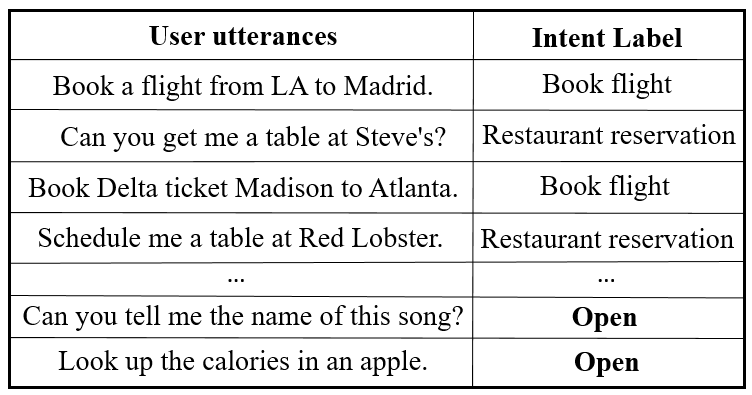
\includegraphics[width=.8\columnwidth]{example.png}
% \centering
% \caption{Three observed trajectories $T_1, T_2, T_3$.}
% \label{trajectories}
% \end{subfigure}

% \begin{subfigure}{\columnwidth}
% \centering
% \includegraphics[width=\columnwidth]{result.png}
% \caption{Learned action models after observing trajectories $T_1, T_2, T_3$ consecutively.}
% \label{action_model}
% \end{subfigure}

% \caption{An example of creating $F(\Pi_{\mathcal{T}})$ from observed trajectories in a logistics domain.}
% \label{example}
% \end{figure}

%%%%%%%%%%%%%%%%%%%%%%%%%%%%%%%%%%%%%%%%% END EXAMPLE %%%%%%%%%%%%%%%%%%%%%%%%%%%%%%%%%%%%%%%%%%%%%%%%%%%%%%%%%%%%%%%%%%%



%%%%%%%%%%%%%%%%%%%%%%%%%%%%%%%%%%%%%%%%%%%%%%% COMPLEXITY ANALYSIS %%%%%%%%%%%%%%%%%%%%%%%%%%%%%%%%%%%%%%%%%%%%%%%%%%%%%%%
\section{Sample Complexity Analysis}

% Background: completeness is an issue
Planning with a safe action model is a sound approach for safe model-free planning, since every plan it outputs is a sound plan according to the real action model. 
However, it is not complete:
a planning problem may be solvable with the real action model, but not the learned one. %action model. 
As in prior work on safe model-free planning~\cite{stern2017efficientAndSafe}, we can bound the likelihood of facing such a problem %by a statistical argument 
as follows. 

% Every action model generated by Algorithm~\ref{alg:sam} is safe, and thus  conservative planning with this action model is \emph{sound}: every generated plan is a sound plan according to the real action model. 
% However, as noted earlier conservative planning is not \emph{complete}: there may exist problems for which any trajectory that solves them is not sound according to the learned action model. 
% For such a problem, we say that the learned 
% In such a case, we say that the learned action model cannot solve these problems. 


% The statistical framework
%Let $f$ denote the number of lifted fluents in the real domain, 
%Let $d$ and $k$ denote the maximum arity (number of parameters) of any lifted fluents and lifted actions, respectively, in the domain. 
Let $\mathcal{P}_D$ be a probability distribution over solvable planning problems in a domain $D$. 
%That is, $\mathcal{P}_D$ is a probability distribution over pairs $\tuple{s_I, s_G}$ where $s_I$ is a state, $s_G$ is a goal condition that is achievable from $s_I$. 
Let $\mathcal{T}_D$ be a probability distribution over pairs $\tuple{P, T}$ 
given by drawing a problem $P$ from $\mathcal{P}(D)$, 
using a sound and complete planner to generate a plan for $P$, 
and setting $T$ to be the trajectory from following this plan.\footnote{%
The planner need not be deterministic.}
 %, respectively.


% Let $\mathcal{D}$ be a probability distribution over tuples of the form $\tuple{s_I, s_G, T}$, where $s_I$ is a state, $s_G$ is a goal condition, and $T$ is a trajectory that is applicable in $s_I$ and ends in a state that satisfies $s_G$, 
% according to a planning domain $D$. 
% The distribution $\mathcal{D}$ implicitly defines a distribution over problems in the domain $D$






\begin{theorem}\label{sam-sample-thm}
Under the injective action binding assumption, given 
%\[
%m \geq \frac{1}{\epsilon} (2\ln 3\sum_{\substack{\text{fluents }F\\\text{ actions } A}}\prod_{\text{types }T}arity(A,T)^{arity(F,T)} + \ln \frac{1}{\delta})
$m \geq \frac{1}{\epsilon} (2\ln 3\sum_{\substack{\liftf\in\mathcal{F}\\\lifta\in\mathcal{A}}}\prod_{t\in T}arity(\lifta,t)^{arity(\liftf,t)} + \ln \frac{1}{\delta})$
%\]
trajectories sampled from $\mathcal{T}_D$, with probability at least $1-\delta $ 
SAM learning for lifted domains (Algorithm~\ref{alg:sam}) returns a safe action model $M_\sam$ such that a problem drawn from $\mathcal{P}_D$ is not solvable with $M_\sam$ with probability at most $\epsilon$.
\end{theorem}
% \begin{theorem}\label{sam-sample-thm}
% Under the injective binding assumption, given $m \geq \frac{1}{\epsilon} (2\ln 3|\mathcal{F}||\mathcal{A}|k^{d} + \ln \frac{1}{\delta})$ trajectories sampled from $\mathcal{T}_D$, then with probability at least $1-\delta $ 
% SAM learning for lifted domains (Algorithm~\ref{alg:sam}) returns a safe action model $M_\sam$ such that the probability of drawing from $\mathcal{P}_D$ a problem that is not solvable with $M_\sam$ is at most $\epsilon$.
% \end{theorem}
Theorem~\ref{sam-sample-thm} guarantees
that with high probability ($\geq 1-\delta$) SAM Learning returns an action model that will only fail to solve a given problem with low probability ($\leq \epsilon$), given a number of example trajectories linear in the size of the models.
%(i.e., \#actions$\times$2$\times$\#possible parameter-bound fluents, since both the preconditions and effects are sets of lifted fluents). 
For example, in the real action model of our simple logistics example with two binary fluents and three ternary actions, the load and unload actions have a single argument of each type; only the move action has two arguments of the same type (location). The only fluents that have location arguments are the at fluents, which have arity one with respect to locations. Thus, guaranteeing $\epsilon=\delta=5\%$ requires only 324 trajectories.
%\roni{The above sentence is not accurate. Preconditions and effects are not lifted fluents, they are parameter-bound literals, which is different since the binding is not param to object, but function param to fluent param. I'm not sure how to change the above sentence, any ideas?}
%\roni{Brendan, what high-level thing can we say about the sample complexity? I think we can say that if the maximal arity of the fluents and actions is much smaller than the number of actions in the domain, the sample complexity is quasi-linear in the number of lifted actions and lifted fluents.} %It is linear in the number of lifted fluents, 
%lcan, with high probability, solve a given problem. 
%learn awith probability higher than $future problems can actually be solved with the safe action model created by SAM Learning with probability $1-\epsilon$. Then given sufficiently many trajectories, with high probability the safe planning problem is solved (with probability $1-\epsilon$) by passing the action model returned by SAM Learning, together with $\tuple{s_I,s_g}$, to any domain independent planner.
The rest of this section is devoted to establishing Theorem~\ref{sam-sample-thm}. 

%, we require several definitions and proving several inter
%\noindent
% Theorem~\ref{safe-sam-thm} guarantees that SAM Learning returns a safe action model, so we focus on establishing that future problems can actually be solved in the action model with probability $1-\epsilon$. Then given sufficiently many trajectories, with high probability the safe planning problem is solved (with probability $1-\epsilon$) by passing the action model returned by SAM Learning, together with $\tuple{s_I,s_g}$, to any domain independent planner.

\begin{definition}[Adequate]
An action model $M$ is {\em $\epsilon$-adequate} if, with probability at most $\epsilon$, a trajectory $T$ sampled from $\mathcal{T}_D$ contains an action triplet $\tuple{s,a,s'}$ where 
$s$ does not satisfy $\pre_M(a)$.\footnote{An action model may not contain any information about some action $a$. 
For the purpose of safe planning this is equivalent to an action model in which the precondition to $a$ can never be satisfied.}
% $a \in A_\epsilon$ and $s$ does not satisfy $pre(a)$.
\end{definition}


\begin{lemma}\label{adequate-lem}
The action model returned by SAM Learning (Algorithm~\ref{alg:sam}) 
given $m$ trajectories (as specified in Theorem \ref{sam-sample-thm})
is $\epsilon$-adequate with probability at least $1-\delta$. 
%\roni{Doesn't this statement need also something about how many samples are needed to get this? (I assume this is the same as the number in the Theorem} I'm a bit running around in circles with myself about how to write this m nicely. Maybe define a m(eps,del)=.... and then say m(Eps,del) everywhere. Anyhow, there is probably some way you usually do this things and so I assume you'll fix all my stupidities. 
\end{lemma}
\noindent
{\em Sketch of proof.} Since the trajectories are are drawn independently, the probability that an action model that is {\em not} $\epsilon$-adequate is consistent with the $m$ trajectories we draw is bounded by $(1-\epsilon)^m\leq\frac{\delta}{\# \text{action models}}$. A union bound over all of the action models that are not $\epsilon$-adequate completes the proof. A complete proof appears in the 
technical report~\cite{juba2021arxiv}.
%supplementary material. % full version. full version.
%\roni{Supplementary material \#2}
%\begin{proof}
%
%%%Consider a precondition $\tuple{\liftl, b_{\liftl,\lifta}}$ in an action model $M_B$ that is not $\epsilon$-adequate.
%
%
%Consider any action model $M_B$ that may be returned by SAM Learning but is not $\epsilon$ adequate. 
%By definition, the probability of drawing a trajectory from $\mathcal{T}_D$ that is inconsistent with $M_B$ is at least $\epsilon$. Thus, the probability of drawing $m$ samples 
%that are consistent with $M_B$ is at most
%\begin{equation}
%    (1-\epsilon)^{m}\leq e^{-m\cdot\epsilon}.
%\end{equation}
%%% at least $\epsilon/3$ a trajectory $T$ is sampled from 
%%% sampled from $\mathcal{T}_D$ such that $T$ contains a triplet $\tuple{s,a,s'}$ where $s$ does not satisfy $\pre(a)$. 
%%% Since $M_B$ is consistent with the given $m$ trajectories, the probability that it is $\epsilon$ adequate is at most $(1-\epsilon/3)^{m}\leq e^{-\epsilon/3\cdot m}$. 
%%% %created by the SAM Learning algorithm trained with more than $m$ trajectories, then it is consistent with all these $m$ trajectories. 
%%%Observe that 
%%%\begin{equation}
%%%  m 
%%%  \geq \frac{3\ln{3}}{\epsilon} |\mathcal{F}||\mathcal{A}|(k^{d} + \log_3 \frac{3|\mathcal{F}||\mathcal{A}|}{\delta}) 
%%%  \geq \frac{1}{\epsilon} (2\ln 3|\mathcal{F}||\mathcal{A}|k^{d} + \ln\frac{1}{\delta})
%%%\end{equation}
%%%Thus, 
%$M_B$ can only be returned if this occurs. For our choice of $m$,
%\begin{multline}
%e^{-m\cdot \epsilon }
%\leq e^{-(2\ln{3}|\mathcal{F}||\mathcal{A}|k^{d} + \ln\frac{1}{\delta})} 
%= \frac{\delta}{3^{2|\mathcal{F}||\mathcal{A}|k^{d}}}
%\label{eq:singleBadModelProb}
%\end{multline}
%Let $B$ be the set of action models that are not $\epsilon$-adequate. 
%By a union bound over $B$, the probability that SAM Learning will return an action model that is not $\epsilon$-adequate 
%is at most $\frac{|B|\delta}{3^{2|\mathcal{F}||\mathcal{A}|k^{d}}}$.
%There are at most $k^{d}$ possible parameter bindings for every pair of lifted fluent and lifted action. 
%Thus, the total number of parameter-bound fluents is $|\mathcal{F}|\cdot k^d$. 
%For each parameter-bound fluent, each precondition or effect will either contain that fluent, or its negation, or neither of them. Thus, the number of possible preconditions and effects for an individual action is $3^{|\mathcal{F}|\cdot k^{d}}$ each. Hence, the number of possible action models is $3^{|\mathcal{A}|\cdot 2|\mathcal{F}|\cdot k^{d}}$. 
%%%Let $B$ be the set of action models that are not $\epsilon$-adequate. 
%Since $B$ is a set of action models, we have that the size of $B$ is at most $3^{2|\mathcal{A}||\mathcal{F}|\cdot k^{d}}$. 
%\roni{What about the number of effects? shouldn't the number of possible action models be double this number, to account for all possible effects?}\brendan{Yes, added this.}
%Therefore, the probability that SAM Learning will return an action model that is not $\epsilon$-adequate is at most $\delta$. 
%%% an 
%%% the precondition of an $\epsilon$-inadequate model is at most $\delta/3$. Thus, the action model returned by SAM Learning is $\epsilon$-adequate with probability at least $1-\delta/3$.
%%% Thus, the probability that of SAM Learning returning $M_B$ is:
%%% \begin{multline}
%%% (1-\epsilon/3)^m 
%%% %\leq e^{-\frac{\epsilon}{3}m} 
%%% \leq e^{-(\ln{3})\cdot (|\mathcal{F}||\mathcal{A}|k^{d} + \log_3\frac{3}{\delta})} 
%%% = \frac{\delta}{3\cdot 3^{|\mathcal{F}||\mathcal{A}|k^{d}}}    
%%% \end{multline}
%%%     \roni{I'm having some trouble with the math here, I need to go back to school}
%%% \[
%%% (1-\epsilon/3)^m \leq e^{-\frac{\epsilon}{3}m} \leq e^{-\ln{3}(f|A|k^{d} + \log_3\frac{3}{\delta})}
%%% %= e^{-\ln{3}|A|f\cdot k^{d}} e^{-\ln{3} \log_3\frac{3}{\delta}}\\ 
%%% = \frac{\delta}{3\cdot 3^{f|A|k^{d}}}.
%%% \]
%%% Observe that $M_B$ will not be returned if such a triplet is contained in the set of trajectories $\mathcal{T}$: otherwise, the falsified literals are removed from $\pre(a)$ and the algorithm does not add literals back to $\pre(a)$. 
%%% Hence, $M_B$ can only be returned by the SAM Learning algorithm if such triplets were never observed in the $m$ trajectories $\mathcal{T}$ independently sampled from $\mathcal{T}_D$. 
%%% Thus, the probability that the algorithm will return any given precondition of an $\epsilon-$inadequate model \roni{I don't get this. The alg. don't return a precondition, it returns an action model. Maybe you mean the alg will return an action model in which such a literal is not assumed to be a precondition or something like that}is at most $(1-\epsilon/3)^m$. Because 
%%% \[
%%% m \geq \frac{3\ln{3}}{\epsilon} |\mathcal{F}||\mathcal{A}|(k^{d} + \log_3 \frac{3|\mathcal{F}||\mathcal{A}|}{\delta}) > \frac{3\ln{3}}{\epsilon} (|\mathcal{F}||\mathcal{A}|k^{d} + \log_3 \frac{3}{\delta}),
%%% \]
%%% we have 
%%% %\begin{math}
%%% \[
%%% (1-\epsilon/3)^m \leq e^{-\frac{\epsilon}{3}m} \leq e^{-\ln{3}(f|A|k^{d} + \log_3\frac{3}{\delta})}
%%% %= e^{-\ln{3}|A|f\cdot k^{d}} e^{-\ln{3} \log_3\frac{3}{\delta}}\\ 
%%% = \frac{\delta}{3\cdot 3^{f|A|k^{d}}}.
%%% \]
%%% %\end{math}
%%% Therefore, by a union bound over the set of $\epsilon$-inadequate models $B$, the probability that the algorithm will return the precondition of an $\epsilon$-inadequate model is at most $\delta/3$. Thus, the action model returned by SAM Learning is $\epsilon$-adequate with probability at least $1-\delta/3$.
%\end{proof}


%\brendan{I think the below is probably subsumed by the above -- if the preconditions of the actions in the trace are satisfied, the precondition cannot be contradictory, and hence the action must have been observed previously. So maybe we don't need the lemma below after all and we can get a better bound. --BJ}
%\roni{Yes, I totally agree, commented it out. I also think the lemma after that is not needed, and this lemma plus the definition of safe action model (=effects are the same as real model if precond hold). I commented both out and added text accordingly. I think also that we shoudl change $\delta/3$ to $\delta$ as you said (I think). If you agree let me know (or just do it)}
%\brendan{did it.}

% \begin{lemma}\label{see-action-lem}
% Let $A_{\epsilon}$ be the set of actions such that each action $a \in A_{\epsilon}$ appears in a trajectory sampled from $D$ with probability at least $\frac{\epsilon}{3 |A|}$. Let $A(\mathcal{T})$ be the set of all actions that appear in any trajectory in $\mathcal{T}$. The probability that $A_\epsilon \subseteq A(\mathcal{T})$ is at least $1-\delta/3$.
% \end{lemma}
% \begin{proof}
% The probability that an action $a\in A_{\epsilon}$ does not appear in a trajectory sampled from $D$ is at most $1-\frac{\epsilon}{3|A|}$.
% Thus, the probability that $a$ does not appear in the set of all actions that appeared in a trace $A(\mathcal{T})$ is at most $(1-\frac{\epsilon}{3|A|})^m$.

% Because 
% \[
% m \geq \frac{3 \ln{3}}{\epsilon} f|A|(k^{d} + \log_3 \frac{3f|A|}{\delta})
% %= \frac{3 \ln{3}}{\epsilon}|A|(f\cdot k^{d} + f\log_3 \frac{3f|A|}{\delta})
% > \frac{3 \ln{3}}{\epsilon}|A|\log_3 \frac{3|A|}{\delta},
% \]
% we have
% \[
% (1-\frac{\epsilon}{3|A|})^m \leq e^{-\frac{\epsilon m}{3|A|}} < e^{-\frac{\epsilon}{3|A|} \frac{3 \ln{3}|A|}{\epsilon}\log_3 \frac{3|A|}{\delta}} = \frac{\delta}{3|A|}.
% \]
% Therefore, by a union bound over the set $A_\epsilon$, we find that all actions $a\in A_{\epsilon}$ appear in $A(\mathcal{T})$ with probability at least $1-\delta/3$.
% \end{proof}


% \begin{lemma}\label{plan-exists-lem}
% If the injective binding assumption holds, the action model returned by SAM Learning is $\epsilon$-adequate, and $A_\epsilon \subseteq A(\mathcal{T})$, a problem $\tuple{s_I,s_g}$ drawn from $D$ is solved by some plan in the returned action model with probability $1-\epsilon$.
% \end{lemma}
% \begin{proof}
% Let $T$, $s_I$, and $s_g$ be, respectively, a trajectory, initial state, and goal sampled from $D$. Since $A_\epsilon \subseteq A(\mathcal{T})$, with probability at least $1-\epsilon/3$, all actions in $T$ are known to the algorithm. By the definition of $\epsilon$-adequate, with probability at least $1-\epsilon/3$, all actions in $T$ are \textit{applicable} (i.e., their learned preconditions hold in all pre-states of $T$). Finally, since by Theorem~\ref{safe-sam-thm} the action models returned by SAM Learning are safe, the actions in $T$ also yield the same post-states. We have by hypothesis that $s_I$ is the initial state of $T$ and the goal is achieved in $T$, so for the final state of $T$ $s_g\subseteq s_G$. Therefore, with overall probability at least $1-\epsilon$, the sequence of actions appearing in $T$ is a plan that solves $\tuple{s_I,s_g}$ in the returned action model.
% \end{proof}

\noindent
{\em Proof of Theorem~\ref{sam-sample-thm}.} 
Let $M$ be an action model returned by SAM Learning given $m$ samples. 
Thus, $M$ is a safe action model (Theorem~\ref{safe-sam-thm}) and it is $\epsilon$ adequate (Lemma~\ref{adequate-lem}). 
Consider a problem $P$ drawn from $\mathcal{P}(D)$, 
and its corresponding pair $\tuple{P, T}$ from $\mathcal{T}(D)$. 
Since $M$ is $\epsilon$-adequate, with probability at least $1-\epsilon$, 
for every action triplet $\tuple{s,a,s'}\in T$ 
$a$ is applicable in $s$, that is, $\pre_M(a)\subseteq s$. 
Since $M$ is a safe action model, we have that $a_M(s)=a_{\realm}(s)=s'$. 
Thus, with probability at least $1-\epsilon$ the trajectory $T$ is consistent with the learned action model $M$, and therefore $P$ can be solved with $M$\hfill$\qed$ 
\medskip
%%%%%%%%%%%%%%%%%%%%%%%%%%%%%%%%%%%%%%%%%%%%%% END PROOF %%%%%%%%%%%%%%%%%%%%%%%%%%%%%%%%%%%%%%%%%%%%%%%%%%%%%%%%%%%%%%%%%%%%%

%The bound in Theorem~\ref{sam-sample-thm} is pessimistic since 
%Lemma~\ref{adequate-lem} often significantly overestimates the number of parameter-bound fluents that need to be considered, especially when the action has many unique parameters of a given type.
%In such a case, the choice of parameter to be bound to the fluent is uniquely determined. Let $arity(\liftf,t)$ and $arity(\lifta,t)$ denote the number of parameters of the lifted fluent $\liftf$ and action $\lifta$, respectively. Then, there are $arity(\lifta, t)^{arity(\liftf, t)}$ ways to bind the parameters of $\liftf$ of type $t$ to the parameters of $\lifta$, and hence $\prod_{t\in T}arity(\lifta, t)^{arity(
%\liftf, t)}$ ways of binding all of the parameters of $\liftf$ to parameters of $\lifta$ (instead of the $k^d$ bound we used previously). Following the same argument otherwise, we obtain:
%\begin{corollary}\label{sam-sample-cor}
%Under the injective binding assumption, given 
%\[
%m \geq \frac{1}{\epsilon} (2\ln 3\sum_{\substack{\text{fluents }F\\\text{ actions } A}}\prod_{\text{types }T}arity(A,T)^{arity(F,T)} + \ln \frac{1}{\delta})
%m \geq \frac{1}{\epsilon} (2\ln 3\sum_{\substack{\liftf\in\mathcal{F}\\\lifta\in\mathcal{A}}}\prod_{t\in T}arity(\lifta,t)^{arity(\liftf,t)} + \ln \frac{1}{\delta})
%\]
%trajectories sampled from $\mathcal{T}_D$, then with probability at least $1-\delta $ 
%SAM learning for lifted domains (Algorithm~\ref{alg:sam}) returns a safe action model $M_\sam$ such that the probability of drawing from $\mathcal{P}_D$ a problem that is not solvable with $M_\sam$ is at most $\epsilon$.
%\end{corollary}
%If we use the bound of this corollary instead, note that the load and unload actions have a single argument of each type; only the move action has two arguments of the same type (location). The only fluents that have location arguments are the at fluents, which have arity one with respect to locations. 
%Consequently, in a simple logistics example with two fluents of arity two and three actions of arity three, guaranteeing $\epsilon=\delta=5\%$ requires only 324 trajectories according to Corollary~\ref{sam-sample-cor}, 
%while according to Theorem~\ref{sam-sample-thm}
%$2,433$ trajectories are needed. 

%\roni{We may want to shrink this significantly. I tried to merge this into the main theorem, but then it because too ugly. Maybe there's a nice way to do this.}






\section{Multiple Action Bindings}
%In this section, we discuss how SAM learning can be modified to handle cases in which the injective action-binding assumption (Definition~\ref{def:injective}) does not hold. 
When the injective action-binding assumption does not hold, 
multiple action parameters are bound to the same object and thus $(b_\lifta)^{-1}$ is not defined. 
As a result, when SAM Learning infers an effect (Rule 3 in Observation~\ref{obs:sam-rules-lifted-general}) it cannot generalize it to be a unique effect of the corresponding lifted action, as done in line~\ref{line:infer-effect} in Algorithm~\ref{alg:sam}. 
This poses a challenge to learning a safe action model, as the information that can be inferred from observing action triplets can be complex.
%, as demonstrated below.

%\subsection{Example}
For example,
% Example: complex inference
consider a lifted action $\lifta(x,y)$.  
Suppose $x$ and $y$ are associated with the same type and $o$ is an object of that type. 
Given the action triplet 
$\tuple{\{~\}, \lifta(o, o), \{\liftl(o)\}}$, 
the agent can infer that $\liftl(o)$ is an effect of the grounded action $\lifta(o, o)$. 
However, the agent cannot accurately infer the effect of the lifted action $\lifta(x,y)$: it can be
 either $\{\liftl(x)\}$, $\{\liftl(y)\}$, or both. 
 Concretely, if $o_1$ and $o_2$ are two different objects from the same type as $o$, 
 the agent cannot determine if applying $\lifta(o_1,o_2)$ will result in a state with
 $\{\liftl(o_1)\}$, $\{\liftl(o_2)\}$, or $\{\liftl(o_1), \liftl(o_2)\}$.
Consequently, any safe action model must not enable groundings of $\lifta$ that bind $x$ and $y$ to different objects, unless $L(x)$ and $L(y)$ both already hold. 

Now, assume the agent is also given the action triplet 
$\tuple{\{\liftl(o_1)\}, \lifta(o_1, o_2), \{\liftl(o_1)\}}$. 
The pre- and post-state are the same, so in Algorithm~\ref{alg:sam} we cannot learn any new effects of $\lifta$ from this triplet. However, we can infer that $\liftl(o_2)$ is not an effect of the grounded action in this triplet. Consequently, the parameter-bound literal $\liftl(y)$ cannot be an effect of the lifted action $\lifta$. 
Thus, this second action triplet does provide useful information: it allow us to infer that 
the lifted action $\lifta(x,y)$ has a parameter-bound effect $\liftl(x)$. 

In a planning task, we might avoid the above by reformulating the domain to satisfy the injective action binding assumption. However, in a learning setup, we do not have control over how the domain is formulated and so the domain we are learning may indeed violate the injective action binding assumption, preventing the application of SAM learning. Next, we describe Extended SAM Learning, which addresses such cases by capturing the form of inference described above. 


\subsection{Extended SAM Learning}
Extended SAM (E-SAM) learning works in two stages. First, it creates 
for every lifted action $\lifta$ a conjunction and a Conjunctive Normal Form (CNF) formula, denoted $\conj_\pre(\lifta)$ and $\cnf_\eff(\lifta)$, that describe a set of constraints for a safe action model. 
Then E-SAM learning generates a safe action model based on these formulas. 


\subsubsection{Safe Action Model Constraints}
$\conj_\pre(\lifta)$ uses atoms of the form 
\ispre($\tuple{\liftl,b_{\liftl,\lifta}}$), which specify that 
$\tuple{\liftl,b_{\liftl,\lifta}}$ is a precondition $\liftl$ in a safe action model. 
Similarly, $\cnf_\eff(\lifta)$ uses atoms of the form 
\iseff($\tuple{\liftl,b_{\liftl,\lifta}}$), 
which specify that $\tuple{\liftl,b_{\liftl,\lifta}}$ is an effect of $\liftl$ in a safe action model. 

Initially, $\conj_\pre(\lifta)$ and $\cnf_\eff(\lifta)$ 
represent that all possible parameter-bound literals are preconditions and there are no effects. 
Then, E-SAM learning iterates over every action triplet $(s, a, s')$ in the given set of trajectories in which $a$ is a grounding of $\lifta$. 
For every such triplet, it applies the inference rules in Observation~\ref{obs:sam-rules-lifted-general} as follows. 

Every parameter-bound literal $\tuple{\liftl,b_{\liftl, \lifta}}$ 
such that $\tuple{\liftl, b_\lifta\circ b_{\liftl,\lifta}}$ is 
not in the pre-state cannot be a pre-condition (Rule 1). So, we remove \ispre$(\tuple{\liftl,b_{\liftl, \lifta}})$ from $\conj_\pre$ for such parameter-bound literals.  
Similarly, every parameter-bound literal $\tuple{\liftl,b_{\liftl, \lifta}}$ 
such that $\tuple{\liftl, b_\lifta\circ b_{\liftl,\lifta}}$ is 
not in the post-state cannot be an effect (Rule 2). So, we add $\neg$\iseff$(\tuple{\liftl,b_{\liftl, \lifta}})$ to $\cnf_\eff$ for such parameter-bound literals.  
Finally, every grounded literal $\tuple{\liftl, b_\liftl}$ in $s'\setminus s$ must be an effect. 
%, and therefore there exists a parameter-bound literal $\tuple{\liftl, b_\lifta\circ b_{\liftl,\lifta}}$ such that $\tuple{\liftl, b_\lifta\circ b_{\liftl,\lifta}}=\tuple{\liftl, b_\liftl}$ (Rule 3). 
So, we add to $\cnf_\eff$ the disjunction over 
all parameter-bound literals
$\tuple{\liftl, b_\lifta\circ b_{\liftl,\lifta}}$ that satisfy $\tuple{\liftl, b_\lifta\circ b_{\liftl,\lifta}}=\tuple{\liftl, b_\liftl}$ (Rule 3).
Once the given trajectories have been processed by the algorithm, 
we simplify the CNF by applying unit propagation and removing subsumed clauses. 
%We provide detailed pseudocode for creating these formulas for a given lifted action in the supplementary material. 
%\roni{Supplementary material \#3}


% Recall that a \emph{prime implicate} is a clause that is entailed by a formula for which no subclause is also entailed. Our final CNF consists of precisely these prime implicates.

% \begin{lemma}\label{unit-prop-complete-lem}
% All prime implicates of this CNF are derived by unit propagation.
% \end{lemma}
% \begin{proof}
% Note that the clauses created by Rule 1 contain only positive literals, and negative literals are only created by Rule 3, which creates unit clauses. Hence, unit propagation is sufficient to capture all possible cut inferences (a.k.a., resolution inferences) from these clauses. 
% %\roni{What are cut inferences? is it the resolution rule? maybe we can use this term and then the connection to the next one is clearer? but maybe I'm just missing terms. Your call.} 
% By the completeness of resolution for prime implicates (see, e.g., \cite[Chapter 13, Exercise 1]{brachman2004}),
% %\roni{Can you add a reference. I know, this is supposed to be basic, but I had to look this up so maybe reviewer will also be like me?} 
% all of the prime implicates of the CNF can be derived by applications of cut. In turn, therefore, unit propagation can also derive all of the prime implicates of this CNF.
% \end{proof}


\subsubsection{Proxy Actions}
The main challenge in creating a safe action model from the generated formulas is the disjunction in $\cnf_\eff$, which represents uncertainty w.r.t to the effects of action. 
To address this, we create a safe action model with a set of proxy actions that ensure every action is only applicable when we know its effects. We achieve this by computing, for each possible subset of the parameter-bound literals in the formulas for a given action, most general unifiers for the literals; in our setting, such unifiers simply identify subsets of the action parameters. Alternatively, if the parameter-bound literal appears in the precondition, then the literal does not need to be included in the unifier, and we know that the corresponding effect will always hold. Hence, since at least one of the unified parameters occurs in the parameter binding of the effect in the true action model, so when the parameters in the set are all bound to the same object (or the literal appears in the precondition), we can guarantee that the corresponding effect literal holds in the post-state.  In more detail, this is done as follows. 

If an action has only unit clauses, we have a single action with the effects indicated by the positive literals. Otherwise, we create a proxy action for all subsets of the parameter-bound literals in non-subsumed non-unit clauses. (The number of proxy actions is thus exponential in the size of the formula of non-unit clauses.) In this proxy action, we identify all of the parameters that appear in the same position of the literals in the subset with the same fluents. Each proxy action has the following set of preconditions and effects: every unit clause in the CNF and every clause in the corresponding subset specifies an effect of the proxy action. For the subset of literals not chosen for this proxy action, the proxy action has the corresponding literals as additional preconditions, in addition to the preconditions of the original SAM Learning action model. 
Every plan generated by the action model created by the resulting action model is translated to a plan without proxy actions by replacing them with the actions for which they were created. 
Algorithms~\ref{alg:esafeplan} and~\ref{alg:extract-clauses} list the complete pseudocode of E-SAM learning. 



\begin{algorithm}[t]
\small
\DontPrintSemicolon
\SetKwInOut{Input}{Input}\SetKwInOut{Output}{Output}
\Input{$\Pi_\mathcal{T} = \tuple{T,O, s_I, G, \mathcal{T}}$}
\Output{$(\pre, \eff)$ for a safe action model}
\BlankLine
    $\mathcal{A'}\gets$ all lifted actions observed in $\mathcal{T}$\\
    \ForEach{lifted action $\lifta\in \mathcal{A'}$}{
        $(\conj_\pre, \cnf_\eff)\gets$ ExtractClauses($\lifta$, $\mathcal{T}(\lifta)$) \nllabel{line:esam:extract-clauses}\\
        $\cnf^1_\eff\gets$ all unit clauses in $\cnf_\eff$\\
        SurelyEff$\gets \{ l ~|~ \text{IsEff}(l)\in \cnf^1_\eff\}$\\
        SurelyPre$\gets \{ l ~|~ \text{IsPre}(l)\in \conj_\pre \}$\\ 
        \tcc{Create proxy actions for non-unit effects clauses}
        $\cnf_\eff\gets \cnf_\eff\setminus \cnf^1_\eff$ \\
        \ForEach{$S\in$ Powerset($\cnf_\eff$)}{
            % $\pre_S, \eff_S \gets$ CreateProxyAction($S$, $\cnf_\eff\setminus S$)\\
            $\pre(\lifta_S)\gets $ SurelyPre; $\eff(\lifta_S)\gets $ SurelyEff \\
            \ForEach{$C_\eff\in \cnf_\eff\setminus S$}{
                \ForEach{$\text{IsEff}(l)\in C_\eff$}{
                    Add $l$ to $\pre(\lifta_S)$
                }
            }
            MergeObjects$\big(S, \pre(\lifta_S),\eff(\lifta_S)\big)$
        }
    } 
    \Return $(\pre, \eff)$ %\nllabel{line:return}
    % \ Let $\mathcal{O} = \{a | a = (pre^U_{\mathcal{T}}(a), eff^L_{\mathcal{T}}(a))\}$ \\
    % \ Define the action model:\\
    % \ $F(\Pi_{\mathcal{T}}) = ((\mathcal{X}, \mathcal{O}), s_I, s_G)$ \\
    % \ Run an off-the-shell classical planner on $F(\Pi_{\mathcal{T}})$ to get the safe plan $\pi$\\
%   \Return{$\pi$}

\caption{Extended SAM Learning}\label{alg:esafeplan}
% \caption{The Safe Action Model (SAM) Learning algorithm}
\end{algorithm}



\begin{algorithm}\small
\DontPrintSemicolon
\SetKwInOut{Input}{Input}\SetKwInOut{Output}{Output}
\Input{$\lifta$, a lifted action}
\Input{$\mathcal{T}(\lifta)$, action triplets that contain $\lifta$}
\Output{$(\conj_\pre, \cnf_\eff)$, representing the constraints over $\pre(\lifta)$ and $\eff(\lifta)$}
\BlankLine
    $\cnf_\eff \gets\emptyset$; $\conj_\pre\gets \emptyset$ \nllabel{line:init}\\ 
    % Add all parameter bound literals
    \ForEach{parameter-bound literal $\tuple{L,b_{\liftl,\lifta}}$}{
        Add \ispre($\tuple{L,b_{\liftl,\lifta}}$) to $\conj_\pre$
    }
    
    \ForEach{$(s, \tuple{\lifta,b_\lifta}, s')\in \mathcal{T}(\lifta)$}{
        % \tcp{Apply Rule 1}
        \ForEach{\ispre($\tuple{L,b_{\liftl,\lifta}}\in \conj_\pre$)}{
            \If{$\tuple{L, b_\lifta\circ b_{\liftl,\lifta}}\notin s$}{
                Remove \ispre($\tuple{L,b_{\liftl,\lifta}}$) from $\conj_\pre$ \nllabel{line:rule1}
            }
        }
    
       % \tcp{Apply Rule 2}
        \ForEach{$\tuple{L,b_\liftl}\in s'\setminus s$}{
            $C_\eff\gets\bot$\\
            \ForEach{$b_{\liftl,\lifta}\in\bindings(b_\lifta, b_\liftl)$}{
                $C_\eff \gets C_\eff \vee$ \iseff($\tuple{\liftl, b_{\liftl,\lifta}})$
            }
            Add EffectsClause to $\cnf_\eff$ \nllabel{line:rule2}
        }
      %  \tcp{Apply Rule 3}
        \ForEach{parameter bound literal $\tuple{L,b_{\liftl,\lifta}}$}{
            $b_\liftl\gets \tuple{L,b_{\liftl,\lifta}\circ b_\lifta}$\\
            \If{$\tuple{L,b_\liftl}\notin s'$}{
                Add $\neg$\iseff($\tuple{L,b_{\liftl,\lifta}}$) to $\cnf_\eff$ \nllabel{line:rule3}
            }
        }
    } 
    Minimize($\cnf_\eff$)~\nllabel{line:minimize}\\
    % Apply unit prop. and subsumption pruning
    \Return $(\conj_\pre, \cnf_\eff)$

\caption{ExtractClauses}
\label{alg:extract-clauses}
\end{algorithm}

% Algorithm~\ref{alg:extract-clauses} creates two Conjunctive Normal Forms (CNFs), denoted $\cnf_\pre(\lifta)$ and $\cnf_\eff(\lifta)$, that describe a set of constraints for the safe action model created by E-SAM Learning. 
% % Then E-SAM learning  generates a safe action model based on these CNFs. 
% $\cnf_\pre(\lifta)$ uses atoms of the form 
% \ispre($\tuple{\liftl,b_{\liftl,\lifta}}$), which specify that 
% $\tuple{\liftl,b_{\liftl,\lifta}}$ is a precondition $\liftl$ in a safe action model. 
% Similarly, $\cnf_\eff(\lifta)$ uses atoms of the form 
% \iseff($\tuple{\liftl,b_{\liftl,\lifta}}$), 
% which specify that $\tuple{\liftl,b_{\liftl,\lifta}}$ is an effect of $\liftl$ in a safe action model. 

% Initially, $\cnf_\pre(\lifta)$ and $\cnf_\eff(\lifta)$ 
% represent that all possible parameter-bound literals are preconditions and there are no effects (line~\ref{line:init}). 
% Then, Algorithm~\ref{alg:extract-clauses} iterates over every action triplet $(s, a, s')$ in the given set of trajectories in which $a$ is a grounding of $\lifta$. 
% For every such triplet, it applies the inference rules in Observation 2 as follows. 
% Every parameter-bound literal $\tuple{\liftl,b_{\liftl, \lifta}}$ 
% such that $\tuple{\liftl, b_\lifta\circ b_{\liftl,\lifta}}$ is 
% not in the pre-state cannot be a pre-condition. 
% So, we remove \ispre$(\tuple{\liftl,b_{\liftl, \lifta}})$ from $\cnf_\pre$ for such parameter-bound literals (line~\ref{line:rule1}).  
% Similarly, every parameter-bound literal $\tuple{\liftl,b_{\liftl, \lifta}}$ 
% such that $\tuple{\liftl, b_\lifta\circ b_{\liftl,\lifta}}$ is 
% not in the post-state cannot be an effect (Rule 2). 
% So, we add $\neg$\iseff$(\tuple{\liftl,b_{\liftl, \lifta}})$ to $\cnf_\eff$ for such parameter-bound literals (line~\ref{line:rule2}).  
% Finally, every grounded literal $\tuple{\liftl, b_\liftl}$ in $s'\setminus s$ must be an effect. 
% So, we add to $\cnf_\eff$ the disjunction over 
% all parameter-bound literals
% $\tuple{\liftl, b_\lifta\circ b_{\liftl,\lifta}}$ that satisfy $\tuple{\liftl, b_\lifta\circ b_{\liftl,\lifta}}=\tuple{\liftl, b_\liftl}$ (line~\ref{line:rule3}).
% Once the given trajectories have been processed by the algorithm, 
% we simplify both CNFs by applying unit propagation and removing subsumed clauses (line~\ref{line:minimize}). 




% \subsection{Proxy Actions and Deleting Effects}

% Note that while observing the action triplet $\tuple{\{~\}, \lifta(o, o), \{\liftl(o)\}}$ 
% does not allow us to infer a unique effect for every application of $\lifta$, 
% it does allow us to infer a unique effect for every application of $\lifta$ in which the two parameters are bound to the same object. 
% To capture this, we create a proxy action $\lifta_{x=y}$ in the learned action model. 
% This action is exactly like $\lifta$ except that it has only a single parameter. 
% The observed action triplet $\tuple{\{~\}, \lifta(o, o), \{\liftl(o)\}}$ 
% can then be converted to use this proxy action$\tuple{\{~\}, \lifta_{x=y}(o), \{\liftl(o)\}}$
% In this action triplet, there is a unique parameter binding and we can infer that the lifted action $\lifta_{x=y}(x)$ has an effect $\liftl(x)$. 
% When using the resulting action model to create a plan, 
% we may get a plan that includes proxy actions. These can then be easily translated back to regular actions by unpacking the parameters as needed. 


% This approach of adding proxy actions requires some additional bookkeeping, since an action with many parameters may spawn multiple proxy actions. Whenever an action triplet for a lifted action $\lifta$ is processed, one needs to also update the action model w.r.t.\ the proxy actions that spawned from it, removing preconditions and adding effects as specified by our inference rules. 
% This may result in some proxy actions becoming redundant. 
% For example, if we observe an action triplet $\tuple{\{~\}, \lifta(o_1, o_2), \{\liftl(o_1)\}}$
% then we can infer that the effect of $\lifta(x,y)$ is to add $\liftl(x)$ and not $\liftl(y)$, 
% and therefore the proxy action $\lifta_{x=y}$ is not needed anymore. 


% In addition, the ``not an effect'' inference rule (Rule 3 in Observation~\ref{obs:sam-rules-lifted-general}) can now be applied to further refine the learned action model. Note that this rule was redundant when the injective action-binding assumption was true, since effects were only added and not removed. 
% However, this rule is useful when the injective action-binding assumption does not hold. 
% For example, applying this rule allows inferring from 
% $\tuple{\{~\}, \lifta(o, o), \{\liftl(o)\}}$ and $\tuple{\{\liftl(o_1)\}, \lifta(o_1, o_2), \{\liftl(o_1)\}}$
% that $\{\liftl(x)\}$ is an effect of $\lifta$. 

% More generally, we store for every lifted action $\lifta$ a Conjunctive Normal Form (CNF) over atoms of the form $\tuple{\liftl,b}\in\eff(\lifta)$ that specifies what was learned about the effects of $\lifta$. 
% Initially, this CNF is empty. 
% Whenever a literal exists in the post-state and not in the pre-state, we add to this CNF a clause that consists of a disjunction over the possible parameter-bound literals that may be an effect, as specified in the ``an effect'' rule (Rule 1). 
% For every parameter-bound literal that does not exist in the post-state, we add its negation to this CNF, as specified in the ``not an effect'' rule (Rule 3). 
% When all the given trajectories have been processed by the algorithm, 
% we simplify this CNF by applying unit propagation and removing subsumed clauses. 

\subsubsection{Theoretical Properties}
E-SAM Learning creates an action model that satisfies the same properties as the action model created by SAM learning under the injective action binding assumption, as captured in Theorems~\ref{safe-sam-thm} and~\ref{thm:sam-learning-complete-grounded}. 

\begin{theorem}\label{extended-sam-safe}
The E-SAM Learning action model is safe.
\end{theorem}
\begin{proof}
For each of the proxy actions, for every effect, at least one of the parameter-bound literals for the identified parameters is an effect of the true action. Furthermore,  the preconditions ensure that the rest of the uncertain effects are already present in the pre-state. The post-state of the proxy action is thus identical to that of the true action when its precondition is satisfied. Likewise, the proxy actions have preconditions that are only stronger than the actual precondition. Eq.~\ref{eq:safe_action_model} therefore holds. The rest of the claim now follows from the argument in Theorem~\ref{safe-sam-thm}.
\end{proof}

Recall that a \emph{prime implicate} is a clause that is entailed by a formula for which no subclause is also entailed. %The created CNF 
$\cnf_\eff$ consists of precisely these prime implicates.
\begin{lemma}\label{unit-prop-complete-lem}
All prime implicates of $\cnf_\eff$ %the CNFs returned by Algorithm~\ref{alg:extract-clauses} 
are derived by unit propagation.
\end{lemma}
\begin{proof}
Note that the clauses created by Rule 3 contain only positive literals, and negative literals are only created by Rule 1 and 2, which create unit clauses. Hence, unit propagation is sufficient to capture all possible resolution inferences from these clauses. 
%\roni{What are cut inferences? is it the resolution rule? maybe we can use this term and then the connection to the next one is clearer? but maybe I'm just missing terms. Your call.} 
By the completeness of resolution for prime implicates (e.g., \cite[Ch.\ 13, Exercise 1]{brachman2004}),
%\roni{Can you add a reference. I know, this is supposed to be basic, but I had to look this up so maybe reviewer will also be like me?} 
all of the prime implicates of $\cnf_\eff$ %the CNF 
can be derived by resolution. In turn, therefore, unit propagation can also derive all of the prime implicates of $\cnf_\eff$.
%this CNF.
\end{proof}



\begin{theorem}\label{e-sam-strong-theorem}
Every action model $M'$ that is consistent with $\mathcal{T}$ 
and safe w.r.t.\ the real action model \realm is also safe with respect to the extended SAM Learning action model.
\end{theorem}
\noindent
\emph{Sketch of Proof.}
Observation~\ref{obs:sam-rules-lifted-general} characterizes
the set of action models consistent with $\mathcal{T}$.
Since $\cnf_\eff$ consists of the prime implicates of this set, $M^*$ could be an action model that uniquely satisfies any one of the literals of any clause of $\cnf_\eff$; therefore, for $M'$ to be safe w.r.t.\ this unknown $M^*$, it must bind the literals in accordance with one of our proxy actions. The argument is now similar to the proof of Theorem~\ref{thm:sam-learning-complete-grounded}; a full proof
appears in the technical report~\cite{juba2021arxiv}.
%supplementary material. % full version. the full version. 
%\roni{Supplementary material \#4}
%\begin{proof}
%Let $M'$ be an action model that is consistent with $\mathcal{T}$ and safe w.r.t.\ \realm, and consider any transition $\tuple{s,\tuple{\lifta,b},s'}$ permitted by $M'$. Consider the set $S$ of literals in $s'\setminus s$ that do not correspond to unit clauses in the CNF created by E-SAM Learning, and the set $\bar{S}$ of literals that are the groundings under $b$ of the effects in the non-unit clauses created by E-SAM learning that are not in $s'\setminus s$. Recall, Observation~\ref{obs:sam-rules-lifted-general} characterizes the set action models consistent with $\mathcal{T}$ and by Lemma~\ref{unit-prop-complete-lem}, no sub-clause of the CNF created by E-SAM learning is entailed by the rules of Observation~\ref{obs:sam-rules-lifted-general}. Therefore, for every literal of every non-unit clause of this CNF, there exists an action model consistent with $\mathcal{T}$ in which that literal is the only satisfied literal of the clause. (Otherwise, a strictly smaller clause would be entailed.) Therefore, for each literal $l\in S$, since $M'$ is safe w.r.t.\ \realm, all of the parameters of $\lifta$ in some clause for this effect must be bound to the objects necessary to obtain $l$ as the corresponding effect. Thus, $b$ must be consistent with at least one of the proxy actions $\lifta_{proxy}$. Furthermore, since the literals in $\bar{S}$ may be effects of $\tuple{\lifta, b}$, if they are not in $s'\setminus s$, they must be in $s$, so the preconditions of $\lifta_{proxy}$ are satisfied as well. Since the E-SAM Learning action model is safe by Theorem~\ref{extended-sam-safe}, the post-state of $\lifta_{proxy}$ is therefore equal to that obtained by the true action model, which is in turn also equal to $s'$ since $M'$ is also safe. $\lifta$ is therefore an application of $\lifta_{proxy}$, and we see that the use of $\lifta$ in $M'$ is safe with respect to the set of proxy actions in the E-SAM Learning action model.
%\end{proof}
% Consider first the 
% Learning a safe action model for a grounded dom
% \begin{itemize}
%     \item Rule 1.  $\forall l \in s\setminus s': l \notin \eff(a)$
%     \item Rule 2.  $\forall l \in s'\setminus s: l \in \eff(a)$
%     \item Rule 3.  $\forall l \notin s: l \notin \pre(a)$
% \end{itemize}   






% More generally, we define the following inference rules, which formally define the knowledge that can be inferred about an action $\lifta$ when observing an action triplet $\tuple{s,a,a'}$:
% \begin{itemize}
%     \item Rule 1. $\forall \tuple{\liftl, b_\liftl} \in s\setminus s': 
%                           \tuple{\liftl, b_\liftl} \notin \eff(\tuple{\lifta, b_\lifta})$
%     \item Rule 2. $\forall \tuple{\liftl, b_\liftl} \in s'\setminus s: 
%                           \tuple{\liftl, b_\liftl} \in \tuple{\lifta, b_\lifta}$
%     \item Rule 3. $\forall \tuple{\liftl, b_\liftl} \notin s: 
%                           \tuple{\liftl, b_\liftl} \notin \pre(\tuple{\lifta, b_\lifta})$
% \end{itemize}     
% Rules 1 specifies that a grounded literal that is in $s$ and is not in $s'$ cannot be an effect of the grounded action that was performed at $s$. Rule 2 specifies the opposite: a grounded literal that is in $s'$ and not in $s$ must be an effect of the grounded action. Rule 3 specifies that a grounded literal that is not in $s$ cannot be a precondition of the performed grounded action. 




% By replacing $l$ with a grounded literal $\tuple{\liftl, b_\liftl}$ 
% and $a$ with a grounded action $\tuple{\lifta, b_\lifta}$, 
% we have Rule 1 as $\tuple{\liftl, b_\liftl} \notin \eff(\tuple{\lifta, b_\lifta})$. 
% What can we learn about effects of the lifted action $\lifta$.
% There exists at least one parameter-bound literal of the form $\tuple{\liftl, b_{\liftl,\lifta}}$
% that is an effect of $\lifta$. 
% This parameter-bound literal must satisfy Eq.~\ref{eq:inferbind}, 
% that is 

% % Inference rules:
% % R1. REMOVE EFF:[[ l(o) in s and not in s' then for every x such that b_a(x)=o, 
% %                                               l(x) not in eff of a(...,x,...)]]
% % R2. REMOVE PRE:[[ l(o) not in s then for every x such that b_a(x)=0 
% %                                               l(x) not in pre of a(....,x,....)]]
% % R3. ADD EFF: [[ l(o) not in s and l(o) in s' then $\vee_{b_a(x)=0} l(x)\in\eff(a)$]]
% To model this, we can create a dummy action $\lifta'$ that has a single parameter. 



% As we show in the following example, inferring a safe action model is not trivial. 
% For example, assume that there is a lifted action $a$ with two parameters $x$ and $y$. 
% We observe $a$ in two action triplets: $\tuple{}$ and $\tuple{}$ RONI SEE COMMENT FOR THE NEAT EXAMPLE

% % % The lifted action: a(x,y)
% % % Objects: o
% % % Literals: l1, l2

% % % Observation #1:
% % % l1(o)
% % % pre-state:
% % % a(o,o)
% % % post-state:
% % % l1(o), l2(o)

% % [[ (l2(x) or l2(y) in eff(a)) ]]
% % [[ Apply a to state s is allowed only iff in every instatiation of its action model we will obtain the same post-state ]]

% % % Observation #2: 
% % % l2(o1)
% % % pre-state:
% % % a(o1,o2)
% % % post-state:
% % % l2(o1)
% % [[ l in s and not in s' then l not in eff]
% % [[ l2(y) not in eff(a) ]]
% % % Observation#1 and Observation #2 ==> l2(x) is an effect, l2(y) is not

% % % Observation #3: 
% % % l2(o1)
% % % pre-state:
% % % a(o1,o2)
% % % post-state:
% % % l2(o1)
% % [[ l in s and not in s' then l not in eff]
% % [[ l2(y) not in eff(a) ]]
% % % Observation#1 and Observation #2 ==> l2(x) is an effect, l2(y) is not


% % % Observation #4: 
% % % not(f(o1))
% % % pre-state:
% % % a(o1,o1)
% % % post-state:
% % % f(o1)
% % f(x) or f(y) is an effect

% % % Observation #5: 
% % % f(o1)
% % % pre-state:
% % % a(o1,o2)
% % % post-state:
% % % not(f(o1))
% % not(f(x)) is an effect


% % Consider the following action a(x,y)
% % eff(a) = f(x) and not(f(y))
% % In theory, one can apply a(o,o). 
% % But the outcome it not defined. 
% % So bad. 
% % [[Assumption: if an action has two parameters of the same type, that have conflicting effects, then you cannot ground it by binding the two parameters to the same object]]



% % Inference rules:
% % R1. REMOVE EFF:[[ l(o) in s and not in s' then for every x such that b_a(x)=o, 
% %                                               l(x) not in eff of a(...,x,...)]]
% % R2. REMOVE PRE:[[ l(o) not in s then for every x such that b_a(x)=0 
% %                                               l(x) not in pre of a(....,x,....)]]
% % R3. ADD EFF: [[ l(o) not in s and l(o) in s' then $\vee_{b_a(x)=0} l(x)\in\eff(a)$]]

% % ADD PRE: NOTHING
% % So far we assumed:
% % 1) There is a unique binding between every fluent used in a precondition or effect to its grounded origin.
% % 2) All preconditions are observed, in particular, no preconditions on the relation between the action paramers 
% % ==> paramx=paramy, or paramx<>paramy.

% % Now we can resolve this....


% % We observed $(s,a_g,s')$. 
% % For each grounded literal $l_g$ not in $s$ and in $s'$
% %     For every object $o$ in $\params(lifted(l_g))$
% %         For every parameter $o'$ in $\params(lifted(a_g))$ of the same type as $o$
      
      
% % Lifted: a(x,y)

% % Obs#1:
% % Observed: a(o,o)
% % Saw in the post-state: f(o) changed to true
% % Three possible modes:
% % eff: f(x), f(y), f(x) and f(y)

% % Obs#2:
% % Observed a(o1,o2) where o1!=o2
% % Obs#2 Case 1: Saw in the post-state: f(o1) changed to true, and f(o2) was false before
% % There two possible models:
% %     f(x) certainly in the effects
% %     f(y) certainly not in the effects

% % Obs#2 Case 2: Saw in the post-state: f(o1) changed to true, and f(o2) was true before
% % There two possible models:
% %     f(x) certainly in the effects
% %     f(y) might be in the effects

% % Obs#
% % Case 1: If we have observed f(y) to be true always before applying action a  
% % Case 2: If we have observed f(y) to be false before applying action a  
% %              Case 2.1: If f(y) changed to true



% % Observation:
% % Before: f(o1),f(o2)   After: f(o1),f(o2)   ==> 
% % Before: f(o1)         After: f(o2)   ==> 
% % Before: f(o2)         After: f(x),f(y)   ==> 


\paragraph{Time complexity}
E-SAM learning can be split into two parts: a \textbf{learning} part, which extracts clauses about the preconditions and effects of the actions (line~\ref{line:esam:extract-clauses} in Alg.~\ref{alg:esafeplan}), and a \textbf{compilation} part that generates a PDDL encoding that can be used by off-the-shelf PDDL planners. The latter involves the creation of the proxy actions. 
The learning part of E-SAM learning can be implemented to run in polynomial time in the number of parameter-bound literals and total number of action triplets, similar to SAM learning. 
The compilation part, however, may run in exponential time due to the 
 inability of PDDL to capture the uncertainty over actions' effects that has been learned (captured by $\cnf_\eff$). 
 Future work may investigate avoiding this exponential step by instead compiling the learned knowledge to a domain encoding for a conformant planner~\cite{bonet2010conformant}. 


% We note that the portion of the algorithm that generates the formulas describing the set of possible action models can be implemented to run in polynomial time in the number of parameter-bound literals and total number of transitions, similar to our algorithm for the injective binding setting. Indeed, we observe that the algorithm only creates one clause for each transition in which an action has more than one parameter bound to the same object. We then only require unit propagation and testing for subsumption of propositional clauses. But, we create a set of proxy actions that is exponential in the number of non-unit clauses for each action, and hence run in exponential time with respect to this formula size. 

% We observe that the proof of Theorem~\ref{e-sam-strong-theorem} seems to require such a large set of proxy actions when using a STRIPS representation, which cannot represent the possible combinations of bindings except by creating an action for each one. Thus, the exponential running time seems to be a consequence of the inability of the STRIPS language to capture this kind of uncertainty about the action model.
% In any case, as action parameters are rarely bound to the same object in most domains, we expect the running time of the algorithm to be reasonable in practice.

% \begin{algorithm}
% \DontPrintSemicolon
% \SetKwInOut{Input}{Input}\SetKwInOut{Output}{Output}
% \Input{$\Pi_\mathcal{T} = \tuple{T,O, s_I, s_g, \mathcal{T}}$}
% \Output{An action model that is safe w.r.t. the action model that generated $\mathcal{T}$}
% \Begin{
%     $\mathcal{A'}\gets$ all lifted actions observed in $\mathcal{T}$\\
%     \ForEach{lifted action $\lifta\in \mathcal{A'}$}{
%         $\eff(\lifta)\gets\emptyset$ \\ 
%         $\pre(\lifta)\gets $ all parameter-bound literals \nllabel{line:init_pre} \\
%         \ForEach{$(s, \tuple{\lifta,b_\lifta}, s')\in \mathcal{T}(\lifta)$}{
%             \ForEach{$\tuple{L,b_{\liftl,\lifta}}\in\pre(\lifta)$}{
%                 \If{$\tuple{L, b_\lifta\circ b_{\liftl,\lifta}}\notin s$}{
%                     Remove $\tuple{L,b_{\liftl,\lifta}}$ from $\pre(\lifta)$ \nllabel{line:remove-pre}
%                 }
%             }
%             \ForEach{$\tuple{L,b_\liftl}\in s'\setminus s$}{
%                 EffectsClause $\gets \emptyset$\\
%                 \ForEach{$b_{\liftl,\lifta}\in\bindings(b_\lifta, b_\liftl)$}{
%                     Add IsEffect($\tuple{\liftl, b_{\liftl,\lifta}}$) to EffectsClause
%                 }
%                 Add EffectsClause to $\eff(\lifta)$
%             }
%             \ForEach{parameter bound literal $\tuple{L,b_{\liftl,\lifta}}$}{
%                 $b_\liftl\gets \tuple{L,b_{\liftl,\lifta}\circ b_\lifta}$\\
%                 \If{$\tuple{L,b_\liftl}\notin s'$}{
%                     Add $\neg$IsEffect($\tuple{L,b_{\liftl,\lifta}}$) to $\eff(\lifta)$
%                 }
%             }
%         }
%     } 
%     \Return $(\pre, \eff)$ \nllabel{line:return}
% }
% \caption{ExtractKnowledgeFromTriplets}\label{safeplan}
% % \caption{The Safe Action Model (SAM) Learning algorithm}
% \label{alg:sam}
% \end{algorithm}



%%%%%%%%%%%%%%%%%%%%%%%%%%%%%%%%%%%%%%%%%%%%%% EXPERIMENT %%%%%%%%%%%%%%%%%%%%%%%%%%%%%%%%%%%%%%%%%%%%%%%%%%%%%%%%%%%%%%%%%%%

\section{Experiments}
Next, we perform an experimental evaluation of SAM Learning over planning problems 
from twelve domains from the IPC~\cite{ipc}. % to learn the real action model. 
Table~\ref{tab:domains} lists the names of these domains, the number of lifted fluents and actions, the largest arity of these lifted fluents and actions, and the largest number of grounded fluents and actions in our dataset. % Maybe too detailed
%Various properties of the domains' complexity are summarized in Table \ref{tab:domains}. 
We have chosen only domains in the IPC benchmarks in which the injective action binding assumption holds. 
%Thus, we only implemented SAM Learning (Algorithm \ref{alg:sam}), which is simpler and faster than E-SAM learning and is guaranteed to produce the same output in these domains (since they only differ when the injective binding assumption does not hold).
For such domains, E-SAM Learning and SAM Learning behave the same. %, so we only report therefore the results of SAM learning. %, as it is simpler to implement. 
%Therefore, we did not implement E-SAM Learning (Algorithm \ref{alg:esafeplan}), since it is more complex and is guaranteed to produce the same output as SAM Learning in these domains (since they only differ when the injective action binding assumption does not hold).


\begin{table}[t]
\centering
\resizebox{\columnwidth}{!}{
\begin{tabular}{lccccrr}
\toprule
            &               \#&             \# &        max &       max &       max &       max \\
            & lifted  & lifted & arity & arity &ground&ground\\
            &fluents&actions&fluents&actions & fluents&actions\\ 
\midrule
% Blocksworld& 5                 & 4                 &2                  &2                    \\
% Ferry       & 5                 & 3                 &2                  &2                    \\
% Floortile   & 10                & 7                 &2                  &4                    \\
% Gripper     & 4                 & 3                 &2                  &3                    \\
% Hanoi       & 3                 & 1                 &2                  &3                    \\
% Npuzzle     & 3                 & 1                 &2                  &3                    \\
% Parking     & 5                 & 4                 &2                  &3                    \\
% Sokoban     & 4                 & 2                 &3                  &5                    \\
% Spanner     & 6                 & 3                 &2                  &4                   \\

Blocks      & 5                 & 4                 &2                  &2  & 182 & 182                  \\
Depot      & 6                 & 5                 &4                  &2  & 75 & 450                  \\
Ferry       & 5                 & 3                 &2                  &2& 75 & 75                    \\
Floortile   & 10                & 7                 &2                  &4 & 40 & 64                   \\
Gripper     & 4                 & 3                 &2                  &3& 42 & 84                    \\
Hanoi       & 3                 & 1                 &2                  &3& 33 & 166                    \\
Npuzzle     & 3                 & 1                 &2                  &3& 80 & 80                    \\
Parking     & 5                 & 4                 &2                  &3  & 182 & 2,184                  \\
Satellite      & 8                 & 5                 &2                  &4  & 75 & 1875                  \\
Sokoban     & 4                 & 2                 &3                  &5& 288 & 564                    \\
Spanner     & 6                 & 3                 &2                  &4  & 12 & 12                  \\
Transport      & 5                 & 3                 &2                  &5  & 870 &  3600                \\

\bottomrule
\end{tabular}
}
\caption{Statistics on the domains in our experiments.}
\label{tab:domains}
\end{table}
%, 



% For N-Puzzle, both methods correctly learned the action model after observing a single $\tuple{s ,a,s'}$ triple in all 10 trials. 
% For Blocksworld, Table \ref{tab:experiment} lists the number of state-action-state triples needed to learn a correct action model over 10 runs, where each run processed the trajectories in a random order. 


\iffalse{
%% The old table below.
\begin{table}[ht]
\small
\centering
\begin{tabular}{|l|c|c|c|c|} 
\hline

            & \multicolumn{2}{c|}{Domain Information} & \multicolumn{2}{c|}{\#  $\tuple{s,a,s'}$ needed}   \\ 
             \cline{2-5}
            & \# Predicates & \# Actions            & SAM          & FAMA~                    \\ 
\hline
Blocksworld &       5         &     4                   &   $8\pm1$           &          $15\pm2$               \\ 
\hline
N-Puzzle    &       3         &        1                &            $1\pm0$  &          $1\pm0$                \\
\hline
\end{tabular}
\caption{Number of action triplets needed by SAM algorithm and FAMA algorithm to learn the true action model.}
\label{tab:experiment}
\end{table}
}\fi
%% OLD table above
%% NEW table below
% \begin{table}[ht]
% \small
% \centering
% \begin{tabular}{|l|c|c|c|c|c|c|c|c|c|c|} 
% \hline
%   \# $\tuple{s,a,s'}$         &
%             6 & 7 & 8 & 9 &$\cdots$& 13 & 14 & 15 & 16 & 17  \\        
% \hline\hline
% SAM &       1 & 1 & 6 & 2 & 0 & 0 & 0 & 0 & 0 & 0 \\ 
% \hline
% FAMA    &       0 & 0 & 0 & 0 & 0 & 3 & 1 & 3 & 1 & 2\\
% \hline
% \end{tabular}
% \caption{\# trials in which SAM Learning and FAMA learned the true Blocksworld action model with a given \# of triples.}
% \label{tab:experiment}
% \end{table}

% \begin{table}[]
% \centering
% \begin{tabular}{@{}lrr|rr@{}}
% \toprule
%             & \multicolumn{2}{c}{Triplets} & \multicolumn{2}{c}{Trajectories} \\ 
% Domain      & FAMA          & SAM          & FAMA            & SAM            \\ \midrule
% % Blocksworld & 44.63         & 24.88        & 2.00            & 1.00           \\
% % Ferry     & 12.75         & 9.75        & 1.00            & 1.00           \\ 
% % Floortile     & 36.50         & 14.50        & 2.00            & 1.00           \\ 
% % Gripper     & 8.25         & 4.75        & 1.00            & 1.00           \\ 
% % Hanoi     & 3.00         & 3.00        & 1.00            & 1.00           \\ 
% % Npuzzle     & 1.00          & 1.00         & 1.00            & 1.00           \\
% % Parking     & 64.25         & 42.50        & 3.50            & 2.00           \\
% % Sokoban     & 7.75         & 5.75        & 1.00            & 1.00           \\ 
% % Spanner     & 19.00         & 17.00        & 1.00            & 1.00           \\ 
% Parking     & 64.25         & 42.50        & 3.50            & 2.00           \\
% Blocksworld & 44.63         & 24.88        & 2.00            & 1.00           \\
% Floortile     & 36.50         & 14.50        & 2.00            & 1.00           \\ 
% Spanner     & 19.00         & 17.00        & 1.00            & 1.00           \\ 
% Ferry     & 12.75         & 9.75        & 1.00            & 1.00           \\ 
% Gripper     & 8.25         & 4.75        & 1.00            & 1.00           \\ 
% Sokoban     & 7.75         & 5.75        & 1.00            & 1.00           \\ 
% Hanoi     & 3.00         & 3.00        & 1.00            & 1.00           \\ 
% Npuzzle     & 1.00          & 1.00         & 1.00            & 1.00           \\
% \bottomrule
% \end{tabular}
% \caption{\ Average number of trajectories and triplets in which SAM Learning and FAMA learned the true action models.}
% \label{tab:experiment}
% \end{table}

\setlength{\tabcolsep}{3pt}
\begin{table}[bt!] % I hate being immodest but I am the king of Latex !!!! :) all it took was this lousy exclamation mark
\centering
\resizebox{\columnwidth}{!}{
\begin{tabular}{ll|cc|cc}
\toprule
                                &                                   & \multicolumn{2}{c}{Trajectories}                   & \multicolumn{2}{c}{Triplets}                       \\ 
Domain                          & \# Objects                        &SAM&FAMA&SAM&FAMA\\\midrule
\multirow{8}{*}{Blocks} & 7 blocks                                & 1                       & 2                        & 13                      & 22                       \\
                                & 8 blocks                                & 1                       & 2                        & 16                      & 29                       \\
                                & 9 blocks                                & 1                       & 2                        & 18                      & 35                       \\
                                & 10 blocks                                & 1                       & 2                        & 22                      & 40                       \\
                                & 11 blocks                                & 1                       & 2                        & 25                      & 46                       \\
                                & 12 blocks                                & 1                       & 2                        & 28                      & 53                       \\
                                & 13 blocks                                & 1                       & 2                        & 35                      & 60                       \\
                                & 14 blocks                                & 1                       & 2                        & 42                      & 72                       \\ \midrule
\multirow{4}{*}{Depot}       & 1 truck, 2 places, 4 hoists, 10 crates& 1                       & 1                        & 18                       & 24                        \\
                                & 1 truck, 2 places, 4 hoists, 15 crates& 1                       & 1                        & 26                       & 32                       \\
                                & 2 trucks, 3 places, 5 hoists, 10 crates& 1                       & 1                        & 22                      & 28                       \\
                                & 2 trucks, 3 places, 5 hoists, 15 crates& 1                       & 1                        & 28                      & 36                       \\ \midrule
\multirow{4}{*}{Ferry}       & 2 locations, 8 cars               & 1                       & 1                        & 4                       & 7                        \\
                                & 3 locations, 10 cars              & 1                       & 1                        & 9                       & 12                       \\
                                & 4 locations, 12 cars              & 1                       & 1                        & 12                      & 15                       \\
                                & 5 locations, 15 cars              & 1                       & 1                        & 14                      & 17                       \\ \midrule
\multirow{4}{*}{Floortile}   & 3x3, 2 robots                     & 1                       & 2                        & 13                      & 22                       \\
                                & 4x3, 2 robots                     & 1                       & 2                        & 13                      & 32                       \\
                                & 4x4, 2 robots                     & 1                       & 2                        & 16                      & 40                       \\
                                & 5x4, 2 robots                     & 1                       & 2                        & 16                      & 52                       \\ \midrule
\multirow{4}{*}{Gripper}        & 2 rooms, 6 balls                  & 1                       & 1                        & 4                       & 8                        \\
                                & 2 rooms, 10 balls                 & 1                       & 1                        & 5                       & 8                        \\
                                & 3 rooms, 8 balls                  & 1                       & 1                        & 5                       & 8                        \\ 
                                & 3 rooms, 14 balls                 & 1                       & 1                        & 5                       & 9                        \\ \midrule
\multirow{4}{*}{Hanoi}       & 3 disks                           & 1                       & 1                        & 3                       & 3                        \\
                                & 4 disks                           & 1                       & 1                        & 3                       & 3                        \\
                                & 5 disks                           & 1                       & 1                        & 3                       & 3                        \\
                                & 6 disks                           & 1                       & 1                        & 3                       & 3                        \\ \midrule
\multirow{3}{*}{Npuzzle}     & 8 tiles                                 & 1                       & 1                        & 1                       & 1                        \\
                                & 15 tiles                                & 1                       & 1                        & 1                       & 1                        \\
                                & 24 tiles                                & 1                       & 1                        & 1                       & 1                        \\ \midrule
\multirow{4}{*}{Parking}     & 3 curbs, 4 cars                   & 2                       & 3                        & 13                      & 20                       \\
                                & 5 curbs, 8 cars                   & 2                       & 4                        & 32                      & 52                       \\
                                & 7 curbs, 12 cars                  & 2                       & 4                        & 53                      & 87                       \\
                                & 8 curbs, 14 cars                  & 2                       & 3                        & 72                      & 98                       \\ \midrule
\multirow{4}{*}{Satellite}     & 2 sats., 4 instrs., 4 modes, 8 dirs.                      & 1                       & 1                        & 20                       & 28                        \\
                                & 4 sats., 4 instrs., 4 modes, 8 dirs.                        & 1                       & 1                        & 20                       & 28                        \\
                                & 5 sats., 5 instrs., 5 modes, 10 dirs.                        & 1                       & 1                        & 24                       & 32                        \\
                                & 5 sats., 5 instrs., 5 modes, 15 dirs.                      & 1                       & 1                        & 26                       & 34                       \\ \midrule\multirow{4}{*}{Sokoban}& 5x5, 2 boxes                      & 1                       & 1                        & 4                       & 6                        \\
                                & 7x7, 2 boxes                      & 1                       & 1                        & 6                       & 8                        \\
                                & 8x8, 3 boxes                      & 1                       & 1                        & 5                       & 7                        \\
                                & 9x9, 3 boxes                      & 1                       & 1                        & 8                       & 10                       \\ \midrule
\multirow{9}{*}{Spanner}     & 10 spanners, 10 nuts, 2 locations & 1                       & 1                        & 14                      & 16                       \\
                                & 10 spanners, 10 nuts, 4 locations & 1                       & 1                        & 16                      & 18                       \\
                                & 10 spanners, 10 nuts, 6 locations & 1                       & 1                        & 18                      & 20                       \\
                                & 11 spanners, 11 nuts, 2 locations & 1                       & 1                        & 15                      & 17                       \\
                                & 11 spanners, 11 nuts, 4 locations & 1                       & 1                        & 17                      & 19                       \\
                                & 11 spanners, 11 nuts, 6 locations & 1                       & 1                        & 19                      & 21                       \\
                                & 12 spanners, 12 nuts, 2 locations & 1                       & 1                        & 16                      & 18                       \\
                                & 12 spanners, 12 nuts, 4 locations & 1                       & 1                        & 18                      & 20                       \\
                                & 12 spanners, 12 nuts, 6 locations & 1                       & 1                        & 20                      & 22                       \\ \midrule\multirow{4}{*}{Transport}& 2 trucks, 5 packages, 10 locations                      & 1                       & 1                        & 16                       & 20                        \\
                                & 2 trucks, 10 packages, 20 locations                     & 1                       & 1                        & 18                       & 22                        \\
                                & 4 trucks, 10 packages, 20 locations                      & 1                       & 1                        & 22                       & 26                        \\
                                & 4 trucks, 15 packages, 30 locations                    & 1                       & 1                        & 24                       & 30                       \\ \bottomrule
\end{tabular}
}
%\caption{S=SAM, F=FAMA. Results are average over problems with the same number of objects. Note that SAM only required 2 trajectories on Parking, and Floortile shows graceful scaling of learning w.r.t.\ the number of objects.}
\caption{Number of trajectories and action triplets needed to learn the real action model in each domain.} 
%S=SAM, F=FAMA. Results are average over problems with the same number of objects. Note that SAM only required 2 trajectories on Parking, and Floortile shows graceful scaling of learning w.r.t.\ the number of objects.}
\label{tab:all_experiments}
\end{table}

For each domain, we generated problems using the problem generator provided in the IPC learning tracks 
and solved them using their true action models with the MADAGASCAR planner~\cite{Rintanen2014MadagascarS} to obtain example trajectories.
These trajectories were broken to action triplets and given to the SAM Learning algorithm one at a time to obtain a safe action model. We halted this process when the learned action model was equivalent to the real model, and report the number of triplets and trajectories given to the algorithm. 
As a baseline, we performed this experiment also with FAMA \cite{aineto19}, which is a modern algorithm for learning action models from trajectories. Note that unlike SAM Learning, FAMA has no safety guarantee. 
In addition, SAM learning runs in time linear in the number of lifted actions, lifted literals, and trajectories, while FAMA runs an automated planner which has an exponential worst-case running time (as planning is PSPACE-complete). SAM learning is only exponential in the maximal number of parameters of each action and literal. Thus, SAM learning can easily scale to very large domains. 



Table~\ref{tab:all_experiments} lists the results of our experiments. The ``\# Objects'' column lists the objects in the problem, and the values under ``Trajectories'' and ``Triplets'' are the number of trajectories and action triplets, respectively, required to learn the correct model. 
In all cases, both methods were able to recover the real action model. 
However, SAM Learning was able to find such a model using at most as many, and often significantly fewer triplets and trajectories. 
For example, for the Floortile problem with 2 robots and a $5\times 4$ floor, SAM learned the correct model with only 16 action triplets while FAMA required 52 action triplets. In fact, in all domains except Parking, SAM Learning learned the correct model with a single trajectory.  
%using at most as many $(s,a,s')$ triplets as FAMA, and frequently far fewer (see Table~\ref{tab:all_experiments}). 
Note that once SAM Learning finds a correct model it will never change it,  since SAM only removes literals that are not satisfied in the pre-state from the preconditions and adds literals that switch values between pre and post-states to the effects. Meanwhile, FAMA might add irrelevant literals or remove correct literals from the preconditons or effects as it processes more action triplets. 

%not add or remove more literals from the preconditions or effects, since SAM only removes literals that are not satisfied in the pre-state from the preconditions and adds literals that switch values between pre and post-states to the effects. Meanwhile, FAMA might add irrelevant literals or remove correct literals from the preconditons or effects as it processes more transitions. %Once the action model matches the true model, solution plans can then be generated using any classical off-the-shelf planner, such as FastDownward \cite{seipp-et-al-zenodo2017} or Madagascar \cite{Rintanen2014MadagascarS}. 
%In near future, we will consider running validation experiments on more complicated IPC domains. 

The code for SAM learning and our experiments is available at \url{https://github.com/hsle/sam-learning}.

%%%%%%%%%%%%%%%%%%%%%%%%%%%%%%%%%%%%%%%%%%%%%% FUTURE WORK %%%%%%%%%%%%%%%%%%%%%%%%%%%%%%%%%%%%%%%%%%%%%%%%%%%%%%%%%%%%%%%%%%%

\section{Related Work}

A variety of notions of \emph{safety} have been considered in RL, for example capturing the ability to reliably return to a home state \cite{moldovan2012safe} or avoiding undesirable states  \cite{turchetta2016,wachi2018safe} while learning about the environment. 
But, these approaches to safe exploration require some kind of strong prior knowledge, either in the form of beliefs about the transition model or knowledge that the safety levels %vary smoothly in the sense that they 
follow a Gaussian process model. 
Such assumptions are reasonable in the low-level motion planning tasks where RL excels, but they do not suit the kind of discrete, high-level problems typically considered in domain-independent planning.
In addition, in these works safety is soft constraint that an algorithm aims to maximize, while in our case safety is a hard constraint.


Our work is part of the growing literature on learning action models for domain-independent planning~\cite{arora2018review}, which includes algorithms such as ARMS~\cite{yang2007learning}, LOCM~\cite{cresswell2013acquiring}, LOCM2~\cite{cresswell2011generalised}, AMAN~\cite{zhuo2013action}, and FAMA~\cite{aineto19}. 
Similar to SAM learning, ARMS~\cite{yang2007learning} also defines rules to infer an action model from a given set of trajectories. 
Our third rule (``must be an effect'') is somewhat similar to their (I.1) rule. 
The other ARMS rules are different, and are designed to \textbf{explain} the observed trajectories in a succinct manner. Thus, the action model created by ARMS may be either under- or over-constrained for this purpose. % (1) may not be safe, and (2) may be overly constrained.
LOCM~\cite{cresswell2013acquiring} and LOCM2~\cite{cresswell2011generalised} 
learn action models by identifying state transitions that are consistent with the observed trajectories. They do not require as input a set of possible lifted fluents or types, and learn from data the relation between objects and types, as well as the relation between actions and types. 
LOCM2 is a heuristic version of LOCM algorithm for learning action models. It does not support domains in which the injective action binding assumption does not hold, or domains where a deleted literal does not appear as a precondition. 
AMAN~\cite{zhuo2013action} is an action-model learning algorithm that is specifically designed to handle noisy observations. It constructs a graphical model and learns the statistical relationship between actions and possible state transitions. 
FAMA~\cite{aineto19} compiles the problem of finding an action model that is consistent with a set of trajectories to a planning problem. The solution to this planning problem is a sequence of ``actions'' that construct an action model. FAMA is more general than SAM or ESAM in the sense that it supports partial observability. 
%On the other hand, as we show experimentally, SAM learning is able to learn an action model with fewer action triplets. 


FAMA, as well as LOCM, LOCM2, and AMAN, aim to create an action model that \textbf{explains} the given trajectories. This can be viewed as a solving an \emph{inductive logic programming}~\cite{muggleton1994inductive} task. 
The action model they generated is only guaranteed to be \textbf{consistent} with the given set of observations.
Our algorithms (SAM and ESAM) provide a stronger guarantee: the action model they create is \textbf{safe} with respect to the real action model ($\realm$). 
A safe action model (Definition~\ref{def:safe_action_model}) is, by definition, consistent with the given trajectories, 
but a consistent action model (Definition~\ref{def:consistent}) may very well be unsafe. For example, consider an action model $M$ in which the effects of all actions are correct (i.e., match the effects in $\realm$) and all actions have no preconditions. This action model is clearly unsafe, and plans generated with it may be unsound. Yet, such an action model is consistent with any trajectory generated according to the real action model ($\realm$). 
None of the above works provide a safety guarantee, and plans generated with the action models they generate may be unsound.\footnote{Note that the soundness and completeness of FAMA (Lemmas 1 and 2 there) do not refer to plans generated by the action model FAMA learns, but to the learning algorithm it self. 
That is, FAMA is sound in the sense that the action model it returns is consistent with the given trajectories, and it is complete in the sense that if a consistent action model exists then FAMA will find it. Indeed, FAMA may return an unsafe action model.}

% the reverse statement is incorrect: 
% Definitions~\ref{def:consistent} and~\ref{def:safe_action_model} clearly distinguish between consistency and safety: 
% but is not necessarily safe. 
% Thus, one may view these prior works as 
% The algorithms we presented create action models that are consistent with the set of given trajectories. Thus, in this sense they can be viewed as solving an \emph{inductive logic programming}~\cite{muggleton1994inductive} task. 
% The safe model learning task, however, generally does not reduce to inductive logic programming: it is important that the model we produce is conservative in certain ways, and not every model consistent with the data would yield a safe action model. In particular, assuming an empty set of preconditions to all actions is consistent with all state-action-state triplets, yet it would not be a safe action model.
% Similar to SAM learning, the ARMS algorithm~\cite{yang2007learning} also defines rules to infer an action model from a given set of trajectories. 
% Our third rule (``must be an effect'') is somewhat similar to their (I.1) rule. 
% %, which states that if a fact   
% However, the ARMS rules are designed to \emph{explain} the observed trajectories in a succinct manner.  Thus, the action model created by ARMS (1) may not be safe, and (2) may be overly constrained.
% [Uncomment if needed] For example, ARMS adds a set of ``Information constraints'', which includes rule (I.3) that sets a literal as a precondition only if it is common enough before some action, thus it may choose not to set a literal to be a precondition even though it does not violate our rule 1 (``not a precondition''). Consequently, the resulting action model may not be safe. 
% On the other hand, ARMS adds a set of ``Plan Constraints'' to ensure the observed trajectories do not contain redundant actions.
% While this is a reasonable assumption, it is may not be true and add unnecessary preconditions. 

\section{Relaxing the Assumptions}

% Preconditions that are k-CNFs
Our learning of preconditions is very similar to Valiant's elimination algorithm \cite{Valiant1984} for learning conjunctions in supervised learning. 
Following his work, we can easily support preconditions that are $k$-CNFs (and not just a simple conjunction) 
by considering that all sets of possible clauses of size $k$ as preconditions instead of a simple conjunction. 
This will increase the sample complexity bound in Theorem~\ref{sam-sample-thm} by raising the first term to the $k^{\text{th}}$ power and similarly increase the running time.
% Conditional effects
Conditional effects can be similarly supported if we can bound the number of literals in their firing condition by some value $k$. 
In this case, the extension to SAM learning keeps track of all possible conditions with at most $k$ literals that hold when an action is applied. 



% The assumption that the preconditions are simple conjunctions can easily be relaxed to allow for $k$-CNF preconditions, for some fixed $k$. 
% This means that the preconditions consist of clauses (of parameter-bound literals) of at most $k$ literals. Indeed, our learning of preconditions is very similar to Valiant's elimination algorithm \cite{Valiant1984} for learning conjunctions in supervised learning, and we simply use an analogous transformation: we consider the set of possible clauses of size k, in place of merely the literals. The first term in the sample complexity bound (in Theorem~\ref{sam-sample-thm}) is raised to the power k, and the running time is similarly increased.



% Random noise
We believe that the algorithm can similarly be extended to handle independent, random noise, provided that either (a) all fluents are corrupted with the same probability or (b) the rate of corruption of each fluent is known. Indeed, this is an example of independent attribute noise, and extensions of Valiant's elimination algorithm to these settings were proposed by Goldman and Sloan~\shortcite{GoldmanS1995} (extending Shackelford and Volper~\citeyear{ShackelfordV1988})
and Decatur and Gennaro~\shortcite{DecaturG1995}, respectively. In the presence of such noise, however, the safety property must be weakened: indeed, since any combination of fluent settings may be observed, albeit with exponentially small probability, we can only expect to guarantee that the action model will be safe with high probability w.r.t.\ the noise. 
% Partial observability [[Roni: not sure what you mean by "sufficiently benign partial information"]]
Likewise, we believe similar guarantees are possible in sufficiently benign partial information settings, following Michael~\shortcite{michael2010partialObservability}.

% Non-deterministic environment
If the environment itself is far from deterministic, then clearly the STRIPS rules we learn would be inappropriate, and a different representation would be necessary. We note that if the environment is stochastic and there is noise of unknown rates that differ across fluents, then it seems to be information-theoretically impossible to learn a safe model (in our sense) even when an adequate set of deterministic rules exists, cf.\ the counterexample of Goldman and Sloan~\shortcite{GoldmanS1995}: we cannot distinguish between a fluent that is just corrupted by observation noise from a fluent that is merely correlated with it.

\section{Conclusion and Future Work}

In this work, we presented the Safe Action Model Learning algorithm for lifted domains.
SAM Learning for lifted domains is guaranteed to return an action model that produces sound plans, 
even without knowing the preconditions and effect of the actions in the domain.   
A theoretical analysis shows that the number of trajectories needed to learn an action model that will solve a given problem with high probability is linear in the potential size of the action model. 
This approach is suitable for most domains in current planning benchmarks, 
where the effects of actions are trivial unless the action parameters are bound to different objects. 
We also discussed how to adapt our algorithm to the case where this assumption does not hold. 
In the future, we aim to 
%consider conditional effects and
%evaluate this algorithm experimentally, measuring its coverage in practice with respect to the number of trajectories it is given under different complicated STRIPS domains. 
%Also, we intend to 
extend safe action-model learning to domains with partial observability and stochasticity. 
%We will also examine its performance on more complicated IPC domains.

\section*{Acknowledgements}
This research is partially funded by NSF awards IIS-1908287, IIS-1939677, and CCF-1718380,
and BSF grant \#2018684 to Roni Stern.

\bibliographystyle{kr}
\bibliography{library}
\end{document}
